%%%%%%%%%%%%%%%%%%%%%%%%%%%%%%%%%%%%%%%%%
% Główny plik pracy
% Szablon pracy dyplomowej
% Wydział Informatyki 
% Zachodniopomorski Uniwersytet Technologiczny w Szczecinie
% autor Joanna Kołodziejczyk (jkolodziejczyk@zut.edu.pl)
% Bardzo wczesnym pierwowzorem szablonu był
% The Legrand Orange Book
% Version 5.0 (29/05/2025)
%
% Modifications to LOB assigned by %JK
%%%%%%%%%%%%%%%%%%%%%%%%%%%%%%%%%%%%%%%%%


%----------------------------------------------------------------------------------------
%	PAKIETY ORAZ PLIKI ZAWIERAJĄCE DEFINICJE STYLI I KONFIGURACJĘ OTOCZEŃ LATEX
%----------------------------------------------------------------------------------------

\documentclass[12pt,fleqn,twoside]{book} % JK Rozmiary czcionek są zgodne z wymaganiami uczelni 
% UWAGA! - wydruk jest dwustronny i jest to zabieg zamierzony

% \usepackage{fix-cm} % Zapewnienie, że wszystkie rozmiary czcionek są dostępne

%%%%%%%%%%%%%%%%%%%%%%%%%%%%%%%%%%%%%%%%%
% Plik konfigurujący
% Szablon pracy dyplomowej
% Wydział Informatyki 
% Zachodniopomorski Uniwersytet Technologiczny w Szczecinie
% autor Joanna Kołodziejczyk (jkolodziejczyk@zut.edu.pl)
% Bardzo wczesnym pierwowzorem szablonu był
% The Legrand Orange Book
% Version 5.0 (29/05/2025)
%
% Modifications to LOB assigned by %JK
%%%%%%%%%%%%%%%%%%%%%%%%%%%%%%%%%%%%%%%%%


%----------------------------------------------------------------------------------------
%	VARIOUS REQUIRED PACKAGES AND CONFIGURATIONS
%----------------------------------------------------------------------------------------

%GEOMETRY
\usepackage[top=3.2cm,bottom=3.5cm,left=2.5cm,right=2.5cm,headsep=1.5ex,bindingoffset=1cm,a4paper]{geometry} % Page margins

% GRAPHICS
\usepackage{graphicx} % Required for including pictures
\graphicspath{{Pictures/}} % Specifies the directory where pictures are stored

% For math equations, theorems, symbols, etc
\usepackage{amsmath,amsfonts,amssymb,amsthm} 

% Customize lists
\usepackage{enumitem} 
\setlist{nolistsep} % Reduce spacing between bullet points and numbered lists
\setlist[itemize]{label=--}

% Required for nicer horizontal rules in tables
\usepackage{booktabs} 

% working in multiple languages
\usepackage{csquotes}

\usepackage{xcolor} % Required for specifying colors by name

% Define blue colors used for highlighting throughout the book- based on the WI ZUT colors
\definecolor{blueWI}{cmyk}{.6,.2,0,.0} % JK - Define the blue colour used for highlighting throughout the book
\definecolor{blueZUT}{cmyk}{1,.75,0,.2} % JK - Define the blue colour used for highlighting throughout the book
\definecolor{grayZUT}{cmyk}{0,0,0,0.4} % JK - Define the blue colour used for highlighting throughout the book

%other definision
\newcommand{\rulecolor}[1]{\color{#1}\rule}


%----------------------------------------------------------------------------------------
%	FONTS AND LANGUAGE (JK - configuring and styling)
%----------------------------------------------------------------------------------------
\usepackage[book]{FiraSans} %% option 'sfdefault' activates Fira Sans as the default text font
\usepackage[T1]{fontenc}
% \usepackage{lmodern}
\renewcommand*\oldstylenums[1]{{\firaoldstyle #1}}

\usepackage{newtxmath,newtxtext}
\usepackage[polish]{babel}% moved after to avoid conflict between polish babel and amsmath
\usepackage[utf8]{inputenc} 
%\usepackage{avant} % Use the Avantgarde font for headings

%----------------------------------------------------------------------------------------
%	PAGE HEADERS AND FOOTERS (JK - Styling for the current chapter in the header)
%----------------------------------------------------------------------------------------

\usepackage{fancyhdr} % Required for header and footer configuration
\setlength{\headheight}{30pt}
\pagestyle{fancy} % Enable the custom headers and footers

\renewcommand{\chaptermark}[1]{\markboth{\sffamily\normalsize\thechapter.\hspace{5pt} #1}{}} % JK - Styling for the current chapter in the header
\renewcommand{\sectionmark}[1]{\markright{\sffamily\normalsize\thesection\hspace{5pt} #1}{}} % Styling for the current section in the header

\fancyhf{} % Clear default headers and footers

% JK - header with page hanging  and chapter title in the box
\fancyhead[EL]{%
  \textcolor{white}{%
    \llap{%
      \colorbox{blueZUT}{%
        \makebox[7ex][r]{\sffamily\thepage}%
      }%
      \hspace{1.25\marginparsep}%
      \hspace{-\fboxsep}%
    }%
    \textcolor{black}{%
      \colorbox{blueWI!20}{%
        \makebox[\textwidth][l]{\sffamily\shorttitle}}}
     \addtolength{\headheight}{5ex} % Increase the spacing around the header slightly
  }%
}
\fancyhead[OR]{%
  \textcolor{white}{%
    \llap{%
      \colorbox{blueZUT}{%
        \makebox[7ex][r]{\sffamily\thepage}%
      }%
      \hspace{1.25\marginparsep}%
      \hspace{-\fboxsep}%
    }%
    \textcolor{black}{%
      \colorbox{blueWI!20}{%
        \makebox[\textwidth][l]{\sffamily\leftmark}}}%{\rightmark}}}
    \addtolength{\headheight}{5ex} % Increase the spacing around the header slightly    
  }%
}

\fancypagestyle{plain}{%
   \fancyhead{} % get rid of headers
   \fancyfoot[RE,RO]{
  	\textcolor{white}{%
    	\llap{%
      	\colorbox{blueZUT}{%
        	\makebox[7ex][l]{\sffamily\thepage}%
      }%
      \hspace{-6\marginparsep}%separation from the margin
      \hspace{-5\fboxsep}%
     }%
     }%
    } 
   \addtolength{\headheight}{18pt} % Increase the spacing around the header slightly
}


\renewcommand*{\headrulewidth}{0pt}
\renewcommand*{\footrulewidth}{0pt}

% Removes the header from odd empty pages at the end of chapters
\makeatletter
\renewcommand{\cleardoublepage}{
\clearpage\ifodd\c@page\else
\hbox{}
\vspace*{\fill}
\thispagestyle{empty}
\newpage
\fi}

%----------------------------------------------------------------------------------------
%	BIBLIOGRAPHY (JK - configuring and styling)
%----------------------------------------------------------------------------------------
% 
\usepackage[
style=numeric,% style alphabetic or numeric
citestyle=numeric,
sorting=nyt,%name -year -title
sortcites=true,
autopunct=true,
autolang=hyphen,
hyperref=true, % if the citation is the link to bibliography
backend=biber,
defernumbers=true]{biblatex}
\addbibresource{bibliography.bib} % BibTeX bibliography file
\defbibheading{bibempty}{}


%\usepackage{calc} % For simpler calculation - used for spacing the index letter headings correctly

%----------------------------------------------------------------------------------------
%	CHAPTER & SECTION HEADINGS
%----------------------------------------------------------------------------------------

\usepackage[explicit]{titlesec}

% \titleformat{<command>}[<shape>]{<format>}{<label>}{<sep>}{<before-code>}[<after-code>]

\titleformat{\chapter}[block]
  {\huge\sffamily\color{blueZUT}}
  {\hspace{-3ex} \thechapter.}
  {0.5em}
  {\parbox[t]{\dimexpr\textwidth-0.5em}{#1\strut}}

\titleformat{name = \chapter, numberless}[block]
  {\huge\sffamily\color{blueZUT}}
  {{#1\strut}}
  {0pt}
  {}[]

%----------------------------------------------------------------------------------------
%	Hanging SECTION NUMBERING (MARGIN)
%----------------------------------------------------------------------------------------

\makeatletter
\renewcommand{\@seccntformat}[1]{\llap{\textcolor{blueZUT}{\csname the#1\endcsname}\hspace{1em}}}                    

\renewcommand{\section}
{\@startsection{section}{1}{\z@}
{-4ex \@plus -1ex \@minus -.4ex}
{1ex \@plus.2ex }
{\normalfont\large\sffamily\bfseries}}

\renewcommand{\subsection}{\@startsection {subsection}{2}{\z@}
{-3ex \@plus -0.1ex \@minus -.4ex}
{0.5ex \@plus.2ex }
{\normalfont\sffamily\bfseries}}

\renewcommand{\subsubsection}{\@startsection {subsubsection}{3}{\z@}
{-2ex \@plus -0.1ex \@minus -.2ex}
{.2ex \@plus.2ex }
{\normalfont\small\sffamily\bfseries}}                        

\renewcommand\paragraph{\@startsection{paragraph}{4}{\z@}
{-2ex \@plus-.2ex \@minus .2ex}
{.1ex}
{\normalfont\small\sffamily\bfseries}}



%----------------------------------------------------------------------------------------
%	MAIN TABLE OF CONTENTS (JK modification: style, indentation, colors,)
%----------------------------------------------------------------------------------------

\usepackage{titletoc} % Required for manipulating the table of contents
\contentsmargin{0cm} % Removes the default margin

% Chapter text styling
\titlecontents{chapter}[1.25cm] % Indentation
{\addvspace{12pt}\large\sffamily} % Spacing and font options for chapters
{\color{blueZUT!60}\contentslabel[\Large\thecontentslabel]{1.25cm}\color{blueZUT}} % JK Chapter number
{\color{blueZUT}}  
{\color{blueZUT!60}\normalsize\;\titlerule*[.5pc]{.}\;\thecontentspage} % Page number

% Section text styling
\titlecontents{section}
	[1.25cm] % Left indentation
	{\addvspace{3pt}\sffamily} % Spacing and font options for sections
	{\contentslabel[\thecontentslabel]{1.25cm}} % Formatting of numbered sections of this type
	{} % Formatting of numberless sections of this type
	{\;\titlerule*[.5pc]{.}\;\color{black}\thecontentspage} % Formatting of the filler to the right of the heading and the page number

% Subsection text styling
\titlecontents{subsection}
	[2.5cm] % Left indentation
	{\addvspace{1pt}\sffamily\small} % Spacing and font options for subsections
	{\contentslabel[\thecontentslabel]{1.25cm}} % Formatting of numbered sections of this type
	{} % Formatting of numberless sections of this type
	{\ \titlerule*[.5pc]{.}\;\thecontentspage} % Formatting of the filler to the right of the heading and the page number

%%%%% JK Add figures and tables
% Figure text styling
\titlecontents{figure}
	[0em] % Left indentation
	{\addvspace{3pt}\sffamily} % Spacing and font options for figures
	{\contentslabel[\thecontentslabel]{1.25cm}} % Formatting of numbered sections of this type
	{} % Formatting of numberless sections of this type
	{\ \titlerule*[.5pc]{.}\;\thecontentspage} % Formatting of the filler to the right of the heading and the page number

% Table text styling
\titlecontents{table}
	[0em] % Left indentation
	{\addvspace{3pt}\sffamily} % Spacing and font options for tables
	{\contentslabel[\thecontentslabel]{1.25cm}} % Formatting of numbered sections of this type
	{} % Formatting of numberless sections of this type
	{\ \titlerule*[.5pc]{.}\;\thecontentspage} % Formatting of the filler to the right of the heading and the page number


%----------------------------------------------------------------------------------------
%	THEOREM STYLES
%----------------------------------------------------------------------------------------

\newcommand{\intoo}[2]{\mathopen{]}#1\,;#2\mathclose{[}}
\newcommand{\ud}{\mathop{\mathrm{{}d}}\mathopen{}}
\newcommand{\intff}[2]{\mathopen{[}#1\,;#2\mathclose{]}}
\renewcommand{\qedsymbol}{$\blacksquare$}
\renewcommand{\thmname}{Twierdzenie}

% Boxed/framed environments
\newtheoremstyle{blueZUTnumbox}% Theorem style name
{0pt}% Space above
{0pt}% Space below
{\normalfont}% Body font
{}% Indent amount
{\small\bf\sffamily\color{blueZUT}}% Theorem head font
{\;}% Punctuation after theorem head
{0.25em}% Space after theorem head
{\small\sffamily\color{blueZUT}\thmname{#1}\nobreakspace\thmnumber{\@ifnotempty{#1}{}\@upn{#2}}% Theorem text (e.g. Theorem 2.1)
\thmnote{\nobreakspace\the\thm@notefont\sffamily\bfseries\color{black}---\nobreakspace#3.}} % Optional theorem note

% \newtheoremstyle{blacknumex}% Theorem style name
% {5pt}% Space above
% {5pt}% Space below
% {\normalfont}% Body font
% {} % Indent amount
% {\small\bf\sffamily}% Theorem head font
% {\;}% Punctuation after theorem head
% {0.25em}% Space after theorem head
% {\small\sffamily{\tiny\ensuremath{\blacksquare}}\nobreakspace\thmname{#1}\nobreakspace\thmnumber{\@ifnotempty{#1}{}\@upn{#2}}% Theorem text (e.g. Theorem 2.1)
% \thmnote{\nobreakspace\the\thm@notefont\sffamily\bfseries---\nobreakspace#3.}}% Optional theorem note

\newtheoremstyle{blacknumbox} % Theorem style name
{5pt}% Space above
{5pt}% Space below
{\normalfont}% Body font
{}% Indent amount
{\small\bf\sffamily}% Theorem head font
{\;}% Punctuation after theorem head
{0.25em}% Space after theorem head
{\small\sffamily\thmname{#1}\nobreakspace\thmnumber{\@ifnotempty{#1}{}\@upn{#2}}% Theorem text (e.g. Theorem 2.1)
\thmnote{\nobreakspace\the\thm@notefont\sffamily\bfseries---\nobreakspace#3.}}% Optional theorem note

% Non-boxed/non-framed environments
\newtheoremstyle{blueZUTnum}% Theorem style name
{5pt}% Space above
{5pt}% Space below
{\normalfont}% Body font
{}% Indent amount
{\small\bf\sffamily\color{blueZUT}}% Theorem head font
{\;}% Punctuation after theorem head
{0.25em}% Space after theorem head
{\small\sffamily\color{blueZUT}\thmname{#1}\nobreakspace\thmnumber{\@ifnotempty{#1}{}\@upn{#2}}% Theorem text (e.g. Theorem 2.1)
\thmnote{\nobreakspace\the\thm@notefont\sffamily\bfseries\color{black}---\nobreakspace#3.}} % Optional theorem note
\makeatother

% Defines the theorem text style for each type of theorem to one of the three styles above
\newcounter{dummy} 
\numberwithin{dummy}{section}
\theoremstyle{blueZUTnumbox}
\newtheorem{theoremeT}[dummy]{Twierdzenie}
\theoremstyle{blueZUTnum}
\newtheorem{exampleT}{Przykład}[chapter]
\theoremstyle{blacknumbox}
\newtheorem{definitionT}{Definicja}[section]


%----------------------------------------------------------------------------------------
%	DEFINITION OF COLORED BOXES
%----------------------------------------------------------------------------------------

\RequirePackage[framemethod=default]{mdframed} % Required for creating the theorem, definition, exercise and corollary boxes

% Theorem box
\newmdenv[skipabove=7pt,
skipbelow=7pt,
backgroundcolor=black!3,
linecolor=blueZUT,
innerleftmargin=5pt,
innerrightmargin=5pt,
innertopmargin=5pt,
leftmargin=0cm,
rightmargin=0cm,
innerbottommargin=5pt]{tBox}


% Definition box
\newmdenv[skipabove=7pt,
skipbelow=7pt,
rightline=false,
leftline=true,
topline=false,
bottomline=false,
linecolor=blueZUT,
innerleftmargin=5pt,
innerrightmargin=5pt,
innertopmargin=0pt,
leftmargin=0cm,
rightmargin=0cm,
linewidth=2pt,
innerbottommargin=0pt]{dBox}	

% Creates an environment for each type of theorem and assigns it a theorem text style from the "Theorem Styles" section above and a colored box from above
\newenvironment{theorem}{\begin{tBox}\begin{theoremeT}}{\end{theoremeT}\end{tBox}}				  
\newenvironment{definition}{\begin{dBox}\begin{definitionT}}{\end{definitionT}\end{dBox}}	
\newenvironment{example}{\begin{exampleT}}{\hfill{\tiny\ensuremath{\blacksquare}}\end{exampleT}}		



%----------------------------------------------------------------------------------------
%	LISTING ENVIRONMENT
%----------------------------------------------------------------------------------------

\usepackage{listings}

%Polish set of letteres accepted in the listings
\lstset{
literate=%
{ą}{{\k{a}}}1
{Ą}{{\k{A}}}1
{ć}{{\'c}}1
{Ć}{{\'{C}}}1
{ę}{{\k{e}}}1
{Ę}{{\k{E}}}1
{ł}{{\l{}}}1
{Ł}{{\L{}}}1
{ń}{{\'n}}1
{Ń}{{\'N}}1
{ó}{{\'o}}1
{Ó}{{\'O}}1
{ś}{{\'s}}1
{Ś}{{\'S}}1
{ż}{{\.z}}1
{Ż}{{\.Z}}1
{ź}{{\'z}}1
{Ź}{{\'Z}}1
}

\renewcommand{\lstlistingname}{\small\sffamily\bfseries\color{blueZUT} Algorytm} % Change default listing caption to Algorthm
\renewcommand{\lstlistlistingname}{Lista \lstlistingname ów}

\definecolor{codegreen}{rgb}{0,0.6,0}
\definecolor{codegray}{rgb}{0.5,0.5,0.5}

\lstdefinestyle{mystyle}{
 %   backgroundcolor=\color{grayZUT!10},   
    basicstyle= \small\fontfamily{lmss}\selectfont,%\footnotesize\fontfamily{cmss}\selectfont,
    commentstyle=\color{codegray},
    keywordstyle=\color{violet},
    numberstyle=\tiny\color{codegray},%numeracja linijek
    identifierstyle={\color{black}},
    numbers=left,%numeracja linijek
    numbersep=10pt,%numeracja linijek
    stringstyle=\color{codegreen},
    breakatwhitespace=true,         
    breaklines=true,                 
    captionpos=b,                    
    %keepspaces=false,                
    %showspaces=false,                
    showstringspaces=false,
    showtabs=true,                  
    tabsize=2,
    frame=leftline,
    rulecolor = \color{blueWI},
    xleftmargin=5ex,
    xrightmargin=5ex
    }
 
\lstset{style=mystyle}

%----------------------------------------------------------------------------------------
% CAPTIONS ( JK - design and implementation)
%----------------------------------------------------------------------------------------

\usepackage{caption}
\captionsetup[figure]{name={\small\sffamily\color{blueZUT} Rysunek}}
\captionsetup[table]{name={\small\sffamily\color{blueZUT} Tabela}}
\captionsetup{font={small,sf,singlespacing}}


%----------------------------------------------------------------------------------------
%	HYPERLINKS IN THE DOCUMENTS
%----------------------------------------------------------------------------------------

\usepackage{hyperref}
%\hypersetup{hidelinks,backref=true,pagebackref=true,hyperindex=true,colorlinks=false,breaklinks=true,urlcolor=blueZUT,bookmarks=true,bookmarksopen=false}
\hypersetup{hidelinks,breaklinks=true,urlcolor=blueZUT,bookmarksopen=false,pdftitle={Title},pdfauthor={Author}}


 % JK - Plik zawierający podstawowe elementy konfigurujące układ dokumentu
% UWAGA! - raczej nie będzie potrzeby zmieniania jego struktury

%%%%%%%%%%%%%%%%%%%%%%%%%%%%%%%%%%%%%%%%%
% Plik z definicjami
% Szablon pracy dyplomowej
% Wydział Informatyki 
% Zachodniopomorski Uniwersytet Technologiczny w Szczecinie
% autor Joanna Kołodziejczyk (jkolodziejczyk@zut.edu.pl)
% Bardzo wczesnym pierwowzorem szablonu był
% The Legrand Orange Book
% Version 5.0 (29/05/2025)
%
% Modifications to LOB assigned by %JK
%%%%%%%%%%%%%%%%%%%%%%%%%%%%%%%%%%%%%%%%%



\def\HRule{\color{blueWI} \rule{\linewidth}{0.6pt}} % horisontal rule in ZUT color

%----------------------------------------------------------------------------------------
% Typ pracy (wybrać właściwy)
%----------------------------------------------------------------------------------------
%\def\degreename{Praca dyplomowa magisterska} 
\def\degreename{Praca dyplomowa inżynierska}
%\def\degreename{Praca dyplomowa licencjacka}

%----------------------------------------------------------------------------------------
% Temat pracy
%----------------------------------------------------------------------------------------
\def\ttitle{Projekt i aplikacja do tworzenia interaktywnego atlasu ptaków występujących w Polsce}
%\def\shorttitle{Szablon pracy dyplomowej inżynierskiej lub magisterskiej  [\dots]} %Jeżeli tytuł pracy jest na tyle długi, że zajmuje 3 linijki to trzeba podać krótszy ekwiwalent do nagłówków stron parzystych
\def\ttitleEng{Design and application for the creation of an interactive atlas of birds in Poland} %temat pracy w j. angielskim


%----------------------------------------------------------------------------------------
% Informacje o autorze
%----------------------------------------------------------------------------------------
\def\authornames{Patryk Rakowski} %imię i nazwisko autora
\def\noalbum{51626}
\def\speciality{Inżynieria oprogramowania} %nazwa specjalności
\def\field{Informatyka} %dziedzina nauki

%----------------------------------------------------------------------------------------
% Informacje o promotorze
%----------------------------------------------------------------------------------------
\def\supname{dr hab. inż. Imed El Fray} %imię i nazwisko promotora
\def\departmentname{Katedra Inżynierii Oprogramowania i Cyberbezpieczeństwa} %nazwa katedry promotora

%----------------------------------------------------------------------------------------
% Informacje o promotorze dodatkowym (odkomentować w razie potrzeby)
%----------------------------------------------------------------------------------------
% \def\supExt{prof. dr hab. inż. Marian Kowalski} %imię i nazwisko promotora
% \def\departmentnameExt{Katedra Grafiki Komputerowej} %nazwa katedry promotora

%----------------------------------------------------------------------------------------
% Data wydania tematu pracy
%----------------------------------------------------------------------------------------
\def\datetitle{03.03.2020}

%----------------------------------------------------------------------------------------
% Rok i miejsce złożenia pracy
%----------------------------------------------------------------------------------------
\def\placesubmit{Szczecin}
\def\yearsubmit{2025}
  % JK - dodatkowe definicje głównie treść strony tytułowej
% UWAGA! - konieczność edycji celem zmiany autora/tematu/dat itp., itd


%----------------------------------------------------------------------------------------
% OTWARCIE DOKUMENTU
%----------------------------------------------------------------------------------------
\begin{document}

%----------------------------------------------------------------------------------------
% STRONA TYTUŁOWA 
%----------------------------------------------------------------------------------------
%%%%%%%%%%%%%%%%%%%%%%%%%%%%%%%%%%%%%%%%%
% Układ strony tytułowej
% Szablon pracy dyplomowej
% Wydział Informatyki 
% Zachodniopomorski Uniwersytet Technologiczny w Szczecinie
% autor Joanna Kołodziejczyk (jkolodziejczyk@zut.edu.pl)
% Bardzo wczesnym pierwowzorem szablonu był
% The Legrand Orange Book
% Version 5.0 (29/05/2025)
%
% Modifications to LOB assigned by %JK
%%%%%%%%%%%%%%%%%%%%%%%%%%%%%%%%%%%%%%%%%

%----------------------------------------------------------------------------------------
%	STRONA TYTUŁOWA - NIE ZMIENIAĆ
%----------------------------------------------------------------------------------------
\begingroup
\firaoldstyle  %Set sans serif fonts for title page
\centering %Center all paragraphs
\thispagestyle{empty} % Suppress headers and footers on the title page

%----------------------------------------------------------------------------------------
%	LOGOTYPY - NIE ZMIENIAĆ
%----------------------------------------------------------------------------------------
    
\includegraphics[scale=.4]{logo5.jpg}\\[.75cm]

%%%
Wydział Informatyki\\[.25cm]
kierunek studiów: \field\\[.25cm]
specjalność: \speciality\\[1.75cm]
%----------------------------------------------------------------------------------------
%	TYP - NIE ZMIENIAĆ
%----------------------------------------------------------------------------------------
{\Large \degreename}\\[1cm]

%----------------------------------------------------------------------------------------
%	TYTUŁ - NIE ZMIENIAĆ
%----------------------------------------------------------------------------------------
% {\color{blueZUT} 
\Large {\bfseries \MakeUppercase  \ttitle }\\[.5cm]% Thesis title
\large {\bfseries \MakeUppercase \ttitleEng} \\[.5cm]% Thesis title in English

%----------------------------------------------------------------------------------------
%	AUTOR - NIE ZMIENIAĆ
%----------------------------------------------------------------------------------------
 % {\color{blueZUT} {
{\large \bfseries \authornames}\\[.5cm]
{nr albumu: \bfseries {\noalbum}}\\[1cm]

%----------------------------------------------------------------------------------------
%	OPIEKUN PRACY - NIE ZMIENIAĆ
%----------------------------------------------------------------------------------------

{\large  Opiekun:}\\[.5cm]
{\large \bfseries{\supname}}\\[.5cm]
{\departmentname}\\[1cm]

%----------------------------------------------------------------------------------------
%	DODATKOWY OPIEKUN PRACY - NIE ZMIENIAĆ
%----------------------------------------------------------------------------------------

\ifdefined\supExt
    {\large Opiekun zewnętrzny:}\\[.5cm]
    {\large \bfseries{\supExt}}\\[.5cm]
    \departmentnameExt
\fi

%----------------------------------------------------------------------------------------
%	DÓŁ STRONY - NIE ZMIENIAĆ
%----------------------------------------------------------------------------------------
~\vfill
\placesubmit, \yearsubmit\\

\endgroup



%----------------------------------------------------------------------------------------
% PUSTA STRONA PO STRONIE TYUŁOWEJ (JK - design and implementation)
%----------------------------------------------------------------------------------------
\newpage
\thispagestyle{empty}
~\vfill

%----------------------------------------------------------------------------------------
%	STRESZCZENIE I SŁOWA KLUCZOWE (1 STRONA) (JK - design and implementation)
%----------------------------------------------------------------------------------------
\newpage
\thispagestyle{empty}
%%%%%%%%%%%%%%%%%%%%%%%%%%%%%%%%%%%%%%%%%
% Specjalna strona pracy ze streszczeniem i abstractem w j. angielskim
% Szablon pracy dyplomowej
% Wydział Informatyki 
% Zachodniopomorski Uniwersytet Technologiczny w Szczecinie
% autor Joanna Kołodziejczyk (jkolodziejczyk@zut.edu.pl)
% Bardzo wczesnym pierwowzorem szablonu był
% The Legrand Orange Book
% Version 5.0 (29/05/2025)
%
% Modifications to LOB assigned by %JK
%%%%%%%%%%%%%%%%%%%%%%%%%%%%%%%%%%%%%%%%%


\begin{center}
\noindent {{\color{blueZUT}\Large\sffamily  {Streszczenie}}}\\[1cm] 
\end{center}

W niniejszej pracy inżynierskiej przedstawiono projekt, implementację oraz wdrożenie kompleksowej aplikacji webowej do tworzenia interaktywnego atlasu ptaków występujących w Polsce. Celem systemu jest wspieranie zarówno profesjonalnych ornitologów, jak i pasjonatów oraz studentów kierunków przyrodniczych w dokumentowaniu i analizie występowania ptaków w terenie. Projektowany system odpowiada na rosnące potrzeby cyfryzacji obserwacji przyrodniczych oraz zapewnia intuicyjne narzędzia do zarządzania danymi biologicznymi.

System został opracowany w architekturze trójwarstwowej, obejmującej frontend w technologii Angular 17, backend oparty na ASP.NET Core 8 oraz relacyjną bazę danych SQLite. Zastosowano nowoczesne wzorce projektowe, takie jak Dependency Injection, Repository Pattern oraz MVC, co zapewnia skalowalność i przejrzystość rozwiązania. Kluczowym elementem interfejsu użytkownika jest mapa interaktywna (Leaflet.js), umożliwiająca geolokalizację obserwacji oraz ich wizualizację w czasie i przestrzeni.
Wśród głównych funkcjonalności aplikacji znajdują się:
\begin{itemize}
	\item system uwierzytelniania i autoryzacji z wykorzystaniem JWT oraz ról użytkowników (administrator, moderator, użytkownik),
	\item możliwość dodawania, edytowania i weryfikacji obserwacji ptaków z uwzględnieniem danych środowiskowych, fotograficznych i lokalizacyjnych,
	\item katalog gatunków ptaków z filtrami taksonomicznymi oraz szczegółowymi informacjami biologicznymi,
	\item panel statystyk i analiz przestrzenno-czasowych obserwacji (m.in. wykresy, mapa cieplna, dane agregowane),
	\item responsywny interfejs graficzny dostosowany do różnych typów urządzeń.
\end{itemize}

Realizacja projektu była równocześnie praktycznym zastosowaniem wiedzy zdobytej w trakcie studiów z zakresu inżynierii oprogramowania oraz doświadczenia zawodowego w branży IT. Praca potwierdza, że przy odpowiednim doborze nowoczesnych narzędzi i technologii możliwe jest stworzenie funkcjonalnego, bezpiecznego i wydajnego narzędzia wspierającego nauki przyrodnicze. Aplikacja może służyć jako fundament dla dalszego rozwoju rozwiązań z zakresu cyfrowej ornitologii oraz analityki ekologicznej.


\vspace{10pt}
\noindent{\bf słowa kluczowe:} ASP.NET Core, Angular, SQLite, geolokalizacja, ornitologia, aplikacja webowa

\vfill

\pagebreak

\begin{center}
\noindent {{\color{blueZUT}\Large\sffamily {Abstract}}}\\[1cm] 
\end{center}
This engineering thesis presents the design, implementation, and deployment of a modern web-based application for creating an interactive atlas of bird species found in Poland. The system supports both professional ornithologists and enthusiasts, as well as students in natural sciences, in documenting and analyzing bird sightings in the field. The solution addresses the growing demand for digital tools in wildlife observation and provides intuitive means for managing biological data.

The system is built upon a three-tier architecture comprising a frontend written in Angular 17, a backend powered by ASP.NET Core 8, and a lightweight relational SQLite database. Modern architectural patterns are applied, including Dependency Injection, Repository Pattern, and MVC, ensuring scalability, maintainability, and modularity. One of the key UI features is an interactive map (Leaflet.js) that allows users to geolocate and visualize bird observations across time and space.
Core functionalities of the application include:
\begin{itemize}
	\item authentication and role-based authorization (Admin, Moderator, User) using JWT,
	\item creation, editing, and moderation of bird observations with environmental, photographic, and geolocation metadata,
	\item a detailed bird catalog with taxonomic filters and biological descriptors,
	\item analytics dashboards with temporal and spatial visualizations (e.g. charts, heatmaps, and summary indicators),
	\item a fully responsive interface optimized for both desktop and mobile devices.
\end{itemize}

The project serves as a practical application of the academic knowledge in software engineering and professional experience in the IT sector. It demonstrates that modern web technologies can be effectively applied to develop robust, efficient, and secure systems supporting environmental research. The developed application provides a valuable foundation for future systems in digital ornithology and ecological analytics.


\vspace{10pt}
\noindent{\bf keywords:} ASP.NET Core, Angular, SQLite, geolocation, ornithology, web application %abstract.tex 
 
%----------------------------------------------------------------------------------------
%	SPIS TREŚCI (JK - design and implementation)
%----------------------------------------------------------------------------------------
\pagestyle{empty}  % Wyłącz stopkę i nagłówek w TOC
\tableofcontents % wyświetl spis
\addtocontents{toc}{\protect\thispagestyle{empty}} % Zachowaj pusty nagłówek i stopkę w TOC
% Wymuszenie rozpoczęcie pierwszego rozdziału na nieparzystej stronie, aby znajdował się po prawej stronie 
\cleardoublepage 
% Ponownie włącz nagłówki i stopki
\pagestyle{fancy} 

%----------------------------------------------------------------------------------------
%	WSTĘP W PRACY DYPLOMOWEJ (JK - design and implementation)
%----------------------------------------------------------------------------------------
\addcontentsline{toc}{chapter}{Wstęp}
%%%%%%%%%%%%%%%%%%%%%%%%%%%%%%%%%%%%%%%%%
% Plik z wstępem do pracy
% Szablon pracy dyplomowej
% Wydział Informatyki 
% Zachodniopomorski Uniwersytet Technologiczny w Szczecinie
% autor Joanna Kołodziejczyk (jkolodziejczyk@zut.edu.pl)
% Bardzo wczesnym pierwowzorem szablonu był
% The Legrand Orange Book
% Version 5.0 (29/05/2025)
%
% Modifications to LOB assigned by %JK
%%%%%%%%%%%%%%%%%%%%%%%%%%%%%%%%%%%%%%%%%


\chapter*{Wstęp}
\index{Wstęp}

\section*{Wprowadzenie}
\index{Wprowadzenie}

We współczesnym świecie, który staje się coraz bardziej cyfrowy, powstaje coraz większe zapotrzebowanie na nowoczesne systemy informatyczne.
Rozwój technologii informacyjnych i komunikacyjnych (ICT)\footnote{ICT - Information and Communications Technology} wspiera dynamiczny rozwój gospodarki oraz umożliwia innowacje w rożnych dziedzinach oraz codzienny życiu.
Wraz z dynamicznym rozwojem technologii webowych pojawiają się nowe możliwości tworzenia nowoczesnych, responsywnych oraz wydajnych aplikacji wspierających procesy biznesowe.

W niniejszej pracy dyplomowej koncentruję się na projektowaniu, doborze technologii z coraz to większego wachlarza dostępnych frameworków \footnote{Framework albo platforma programistyczna – szkielet do budowy aplikacji. Definiuje on strukturę aplikacji oraz ogólny mechanizm jej działania, a także dostarcza zestaw komponentów i bibliotek ogólnego przeznaczenia do wykonywania określonych zadań. Programista tworzy aplikację, rozbudowując i dostosowując poszczególne komponenty do wymagań realizowanego projektu, tworząc w ten sposób gotową aplikację. } oraz implementacji aplikacji wykonanej w technologii web.

Projekt został zrealizowany w oparciu o framework Angular w części frontendowej, ASP.NET Core dla backendu oraz bazę danych SQLite.

\section*{Cel pracy}
\index{Cel pracy}

Głównym celem pracy jest zaprojektowanie i wdrożenie kompleksowej aplikacji webowej do tworzenia interaktywnego atlasu ptaków, które spełnia wymagania stawiane nowoczesnym systemom oraz aktualne standardy branży, uwzględniając aspekty takie jak:
\begin{itemize}
    \item responsywność i dostępność na różnych urządzeniach,
    \item wydajność i optymalizacja działania,
    \item bezpieczeństwo danych użytkowników,
    \item łatwość w utrzymaniu i rozwijaniu aplikacji.
\end{itemize}

\section*{Zakres pracy}
\index{Zakres pracy}

Praca obejmuje następujące etapy: z części teoretycznej prezentującej zagadnienie aplikacji webowej oraz dobór odpowiednich technologii i narzędzi oraz projekt systemu,
z części praktycznej, która obejmuje implementacje poszczególnych komponentów aplikacji oraz wdrożenie systemu na serwerze produkcyjnym.

Warte podkreślenia jest, że realizacja projektu stanowi praktyczne zastosowanie teorii z zakresu inżynierii oprogramowania oraz zdobytej wiedzy i doświadczenia na studiach
oraz w trakcie praktyk zawodowych i pracy w branży IT. Ponadto, projekt ten stanowi przykład zastosowania nowoczesnego stacku technologicznego, którego znajomość przez specjalistów IT jest coraz bardziej ceniona i pożądana w branży.

\section*{Struktura pracy}
\index{Struktura pracy}

Praca jest podzielona na następujące rozdziały, które skupiają się na poszczególnych etapach tworzenia systemu:

\begin{enumerate}
	\item Analiza wymagań i założeń projektowych.
	\item Wybór i uzasadnienie technologii
	\item Projekt
	\item Implementacja
	\item Wdrożenie
\end{enumerate}

% Wstęp powinien być nie dłuższy niż 2 strony. Najlepiej napisać go dopiero, gdy praca jest już skończona i wszystkie jej części spisane.

% Wstęp powinien zawierać:

% \begin{enumerate}
% \item Opis dziedziny jakiej dotyczy praca, ze wskazaniem, że temat pracy jest ważny, bieżący, itp.
% \item Jaki problem z dziedziny się rozwiązuje.
% \item Cel i teza pracy
% \item W jaki sposób cel zostanie osiągnięty a tez potwierdzona.
% \item Struktura pracy.
% \end{enumerate}  % introduction.tex zawiera treść wstępu

%----------------------------------------------------------------------------------------
%	ROZDZIAŁ 1
%----------------------------------------------------------------------------------------
%%%%%%%%%%%%%%%%%%%%%%%%%%%%%%%%%%%%%%%%%
% Szablon pracy dyplomowej
% Wydział Informatyki 
% Zachodniopomorski Uniwersytet Technologiczny w Szczecinie
% autor Joanna Kołodziejczyk (jkolodziejczyk@zut.edu.pl)
% Bardzo wczesnym pierwowzorem szablonu był
% The Legrand Orange Book
% Version 5.0 (29/05/2025)
%
% Modifications to LOB assigned by %JK
%%%%%%%%%%%%%%%%%%%%%%%%%%%%%%%%%%%%%%%%%

%----------------------------------------------------------------------------------------
%	CHAPTER 1
% 	author: Patryk Rakowski (rp51626@zut.edu.pl)
%----------------------------------------------------------------------------------------

\chapter{Analiza wymagań i założeń projektowych}
\label{rozdzial1}

\section{Analiza potrzeb użytkowników}
\index{Analiza potrzeb użytkowników}

\subsection{Identyfikacja grupy docelowej}
\index{Identyfikacja grupy docelowej}

Jednym z najważniejszych etapów w projektowaniu systemu informatycznego jest identyfikacja grupy docelowej użytkowników.
Po analizie rynku i dostępnych rozwiązań można wyróżnić kilka kluczowych grup użytkowników:
\begin{itemize}
	\item \textbf{Profesjonalni Ornitolodzy\footnote{Ornitologia – dział zoologii zajmujący się ptakami. Domeną zainteresowania ornitologów jest przede wszystkim biologia ptaków, ale także ich zwyczaje, trasy przelotów, gniazdowanie, życie społeczne, obserwacja w terenie itp.}} - osoby zajmujące się nauką i badaniem ptaków zawodowo, główna grupa użytkowników wykorzystujących systemy informatyczne do gromadzenia i analizy danych.
	\item \textbf{Amatorzy i hobbyści} - grupa która interesuje się ptakami w wolnym czasie, lub osoby które chcące rozwijać swoją wiedzę. Często korzystają z aplikacji do identyfikacji lub dokumentacji napotkanych ptaków.,
	\item \textbf{Studenci kierunków przyrodniczych} - studenci biologii, ekologii lub innych kierunków przyrodniczych, którzy mogą korzystać z systemów do nauki i badań terenowych.
	\item \textbf{Badacze i naukowcy} - grupa zbliżona zawodowo do profesjonalnych ornitologów, jednak często badająca inne aspekty związane z ptakami i środowiskiem życia.
\end{itemize}

\subsection{Role i uprawnienia użytkowników}
\index{Role i uprawnienia użytkowników}

W systemach informatycznych istotnym aspektem jest zarządzanie rolami i uprawnieniami użytkowników. W przypadku omawianego systemu można wyróżnić następujące role:
\begin{itemize}
	\item \textbf{Administrator} - osoba odpowiedzialna za zarządzanie systemem, użytkownikami, konfiguracje, utrzymanie.
	\item \textbf{Użytkownik} - osoba korzystająca z systemu do identyfikacji ptaków, dokumentacji obserwacji i przeglądania dostępnych zasobów.
	\item \textbf{Moderator} - osoba odpowiedzialna za sprawdzanie i moderowanie treści wprowadzanych przez użytkowników.
\end{itemize}

\subsection{Profil technologiczny użytkowników}
\index{Profil technologiczny użytkowników}

Użytkownicy charakteryzują się zróżnicowanym poziomem zaawansowania technologicznego, co powinno zostać uwzględnione w procesie projektowym. Interfejsu powinny być proste w obsłudze oraz czytelne.

Spora część użytkowników wciąż głównie korzysta z komputerów osobistych do obsługi systemów biznesowych - czy to w domu czy w miejscu pracy. Jednak nie można zapomnieć o urządzeniach mobilnych, które coraz bardziej zastępują nam komputery w codziennym życiu. Interfejs systemu powinien być dostosowany zarówno dla dużych ekranów komputerowych jak i do małych, wąskich i podłużnych wyświetlaczy telefonów.

\section{Specyfikacja funkcjonalna}
\index{Specyfikacja funkcjonalna}

Celem projektu jest stworzenie aplikacji internetowej umożliwiającej użytkownikom dodawanie ptaków, obserwacji i przeglądanie dostępnych treści. System ma za zadanie wspierać amatorów jak i zaawansowanych ornitologów i badaczy w dokumentowaniu i analizie występowania różnych gatunków ptaków w Polsce.
Poniżej przedstawiono wymagania funkcjonalne systemu:

\subsection{Użytkownicy}
\begin{itemize}
	\item \textbf{Rejestracja i logowanie użytkowników} - system umożliwia rejestracje nowych użytkowników oraz logowanie do aplikacji.
	\item \textbf{Zarządzenie użytkownikami} - system umożliwia administratorom zarządzanie kontami użytkowników.
	\item \textbf{Zarządzanie swoim kontem} - system umożliwia użytkownikom zarządzanie swoim kontem: zmianę adresu e-mail, hasła oraz dezaktywacje konta.
\end{itemize}

\subsection{Strona główna i mapa}
\begin{itemize}
	\item \textbf{Mapa obserwacji} - system udostępnia mapę obserwacji ptaków z zaznaczonymi poszczególnymi obserwacjami.
	\item \textbf{Filtrowanie danych} - mapa umożliwia filtrowanie obserwacji po roku, tygodniu oraz gatunkach ptaków.
	\item \textbf{Szczegóły obserwacji} - znaczniki na mapie przenoszą użytkowników do strony obserwacji której dotyczą.
\end{itemize}

\subsection{Obserwacje}
\begin{itemize}
	\item \textbf{Strona obserwacji} - system udostępnia użytkownikom stronę z zweryfikowanymi obserwacjami ptaków.
	\item \textbf{Filtrowanie danych} - system umożliwia filtrowanie danych na stronie obserwacji po zakresie dat oraz gatunkach ptaków.
	\item \textbf{Dodawanie nowych obserwacji} - system umożliwia dodawanie nowych obserwacji niezweryfikowanych zarejestrowanym użytkownikom. Obserwacja składa się z następujących danych:
	\begin{itemize}
		\item wybór ptaka,
		\item data obserwacji,
		\item liczba osobników,
		\item warunki pogodowe,
		\item siedlisko,
		\item opis,
		\item lokalizacja geograficzna,
		\item zdjęcia.
	\end{itemize}
	\item \textbf{Strona szczegółów obserwacji} - system udostępnia dla każdej obserwacji stronę ze szczegółami danej obserwacji.
		Moderator lub użytkownik który dodał daną obserwację może edytować jej dane lub ją usunąć.
	\item \textbf{Moderacja obserwacji} - strona obserwacji udostępnia moderatorom zakładkę z obserwacjami niezweryfikowanymi oraz możliwość weryfikacji danej obserwacji poprzez podstronę szczegółów obserwacji.
\end{itemize}

\subsection{Ptaki}
\begin{itemize}
	\item \textbf{Strona ptaków} - system udostępnia użytkownikom stronę z zweryfikowanymi ptaków.
	\item \textbf{Filtrowanie danych} - system umożliwia wyszukiwanie ptaków po:
		\begin{itemize}
			\item nazwie,
			\item nazwie naukowej,
			\item rodzinie,
			\item rzędzie,
			\item rodzajowi,
			\item gatunkowi.
		\end{itemize}
	\item \textbf{Dodawanie nowych ptaków} - system umożliwia dodawanie nowych ptaków niezweryfikowanych zarejestrowanym użytkownikom. Ptak składa się z następujących danych:
	\begin{itemize}
		\item nazwa,
		\item nazwa naukowa,
		\item zdjęcie,
		\item rodzina,
		\item rząd,
		\item rodzaj,
		\item gatunek,
		\item status ochrony,
		\item siedlisko,
		\item dieta,
		\item rozmiar,
		\item waga,
		\item rozpiętość skrzydeł,
		\item długość życia,
		\item sezon lęgowy,
		\item opis.
	\end{itemize}
	\item \textbf{Strona szczegółów ptaka} - system udostępnia dla każdego ptaka stronę ze szczegółami danego ptaka.
		Moderator lub użytkownik który dodał danego ptaka może edytować jego dane lub go usunąć.
	\item \textbf{Moderacja ptaków} - strona ptaków udostępnia moderatorom zakładkę z ptakami niezweryfikowanymi oraz możliwość weryfikacji danego ptaka poprzez podstronę szczegółów obserwacji.
\end{itemize}

\subsection{Statystyki}
System udostępnia stronę statystyk obserwacji ptaków. Strona zawiera informację takie jak:
\begin{itemize}
	\item \textbf{Panel główny} z kluczowymi wskaźnikami:
		\begin{itemize}
			\item całkowita liczba zaobserwowanych ptaków,
			\item liczba różnych gatunków ptaków,
			\item najczęściej spotykane gatunki,
			\item najrzadziej spotykane gatunki.
		\end{itemize}
	\item \textbf{Wykresy i wizualizacje}
		\begin{itemize}
			\item mapa cieplna pokazująca najczęstsze lokalizacje obserwacji,
			\item wykres liniowy pokazujący trendy obserwacji w czasie.
		\end{itemize}
\end{itemize}

\section{Wymagania niefunkcjonalne}
\index{Wymagania niefunkcjonalne}

Wymagania niefunkcjonalne definiują cechy systemu, które wpływają na jakość, wydajność oraz użyteczność. Poniżej zostały przedstawione kluczowe wymagania niefunkcjonalne projektowanego systemu:

\subsection{Wydajność i skalowalność}
\begin{itemize}
	\item \textbf{Czas odpowiedzi} - system powinien realizować żądania użytkowników w czasie poniżej 2 sekund.
	\item \textbf{Skalowalność} - architektura systemu powinna umożliwiać skalowanie w przypadku wzrostu liczby użytkowników.
\end{itemize}

\subsection{Bezpieczeństwo}
\begin{itemize}
	\item \textbf{Uwierzytelnianie} - system wykorzystuje bezpieczne uwierzytelnianie sesji użytkowników z użyciem JWT\footnote{JSON Web Token (JWT) to otwarty standard (RFC 7519), który definiuje kompaktowy i samodzielny sposób bezpiecznego przesyłania informacji między stronami jako obiektu JSON. Te informacje mogą być weryfikowane i można im ufać, ponieważ są podpisane cyfrowo. JWT mogą być podpisywane przy użyciu klucza tajnego (z algorytmem HMAC) lub pary kluczy publiczny/prywatny przy użyciu RSA lub ECDSA. Z angl. \cite{jwt.io}}.
	\item \textbf{Autoryzacja} - system implementuje role użytkowników (administrator, moderator, użytkownik) z odpowiednimi uprawnieniami.
	\item \textbf{Ochrona danych} - wrażliwe dane użytkowników muszą być szyfrowane.
\end{itemize}

\subsection{Dostępność i użyteczność}
\begin{itemize}
	\item \textbf{Responsywność} - interfejs użytkownika powinien być w pełni responsywny i dostosowany do wyświetlania na różnych urządzeniach.
	\item \textbf{Intuicyjność} - interfejs powinien być intuicyjny i prostu w użyciu dla szerokiej gamy użytkowników.
\end{itemize}

\subsection{Techniczne}
\begin{itemize}
	\item \textbf{Standardy kodowania} - kod powinien być zgodny z przyjętymi w branży standardami kodowania takimi jak: clean code
	\footnote{Pisanie czystego, zrozumiałego i łatwego w utrzymaniu kodu. Z angl. \cite{freecodecamp.cleancode} \cite{theartofclieancode}}, SOLID
	\footnote{Zasady SOLID to pięć podstawowych wytycznych, które usprawniają projektowanie oprogramowania, sprawiając, że kod jest łatwiejszy w utrzymaniu i skalowalny. Zasada pojedynczej odpowiedzialności (SRP) Zasada otwarta/zamknięta Zasada substytucji Liskova (LSP) Zasada segregacji interfejsu (ISP) Zasada odwrócenia zależności (DIP). Z angl. \cite{geeksforgeeks.solid}}
	oraz standardami dla Angular \cite{Angular_17_Documentation} i ASP.NET Core \cite{ASP.NET_Core_Documentation}
\end{itemize}

\subsection{Wnioski z analizy}

Projektowany system, czerpiąc inspiracje z dostępnych konkurencyjnych rozwiązań, wykorzystując aktualne trendy technologiczne, wprowadza innowacyjne podejście do analizy, dokumentowania i dostępności danych ornitologicznych zarówno dla amatorów jak i profesjonalistów.
 % chapter1.tex zawiera treść rozdziału 1

%----------------------------------------------------------------------------------------
%	ROZDZIAŁ 2
%----------------------------------------------------------------------------------------
%%%%%%%%%%%%%%%%%%%%%%%%%%%%%%%%%%%%%%%%%
% Szablon pracy dyplomowej
% Wydział Informatyki 
% Zachodniopomorski Uniwersytet Technologiczny w Szczecinie
% autor Joanna Kołodziejczyk (jkolodziejczyk@zut.edu.pl)
% Bardzo wczesnym pierwowzorem szablonu był
% The Legrand Orange Book
% Version 5.0 (29/05/2025)
%
% Modifications to LOB assigned by %JK
%%%%%%%%%%%%%%%%%%%%%%%%%%%%%%%%%%%%%%%%%


%----------------------------------------------------------------------------------------
%	CHAPTER 2
%----------------------------------------------------------------------------------------
\chapter{Wybór i uzasadnienie technologii}
\label{rozdzial2}

W tej sekcji zostało przedstawione przegląd i porównanie dostępnych technologii webowych oraz uzasadniony ich wybór w implementacji systemu.

\section{Analiza dostępnych rozwiązań technologicznych}
\index{Analiza dostępnych rozwiązań technologicznych}

\subsection{Frameworki frontendowe}
Poniżej zostało przedstawione porównanie głównych frameworków frontendowych.\cite{reactvsvuevsangularvsnextjs}

\subsubsection{Angular}
Kompletny framework utrzymywany przez Google. Angular wymusza strukture z dużym naciskiem na TypeScript, RxJS i skalowalną architekturę.
\begin{itemize}
	\item \textbf{Język} - TypeScript,
	\item \textbf{Kluczowe cechy} - wstrzykiwanie zależności\footnote{Wstrzykiwanie zależności – wzorzec projektowy i wzorzec architektury oprogramowania polegający na usuwaniu bezpośrednich zależności pomiędzy komponentami na rzecz architektury typu plug-in. Polega na przekazywaniu gotowych, utworzonych instancji obiektów udostępniających swoje metody i właściwości obiektom, które z nich korzystają.}, RxJS\footnote{RxJS to biblioteka do programowania reaktywnego przy użyciu Observables, aby ułatwić tworzenie kodu asynchronicznego lub opartego na wywołaniach zwrotnych. Z ang. \cite{rxjs.dev}}, routing, testowanie, CLI\footnote{CLI to skrót od „Command Line Interface” (interfejs wiersza poleceń). Jest to sposób interakcji użytkownika z komputerem poprzez wprowadzanie poleceń tekstowych w terminalu lub wierszu poleceń, zamiast korzystania z interfejsu graficznego (GUI).},
	\item \textbf{Przypadki użycia} - Aplikacje dla przedsiębiorstw, narzędzia wewnętrzne, sektory regulowane.
\end{itemize}

Zalety:
\begin{itemize}
	\item Kompleksowe rozwiązanie,
	\item Wbudowany system zarządzania stanem (RxJS),
	\item Sile typowanie dzięki wykorzystaniu TypeScript,
	\item Oficjalna biblioteka komponentów (Material),
	\item Dependency injection wbudowany w framework,
	\item Oficjalne wsparcie od Google,
	\item Długoterminowe wsparcie (LTS),
	\item Bogata dokumentacja i duża społeczność.
\end{itemize}

Wady:
\begin{itemize}
	\item Wysoki próg wejścia,
	\item Większy rozmiar aplikacji w porównaniu do innych frameworków,
	\item Mniej elastyczny niz React,
	\item Wymaga znajomości wielu konceptów inżynierii oprogramowania,
	\item Mniejsza ilość dostępnych komponentów niż w React.
\end{itemize}

\subsubsection{React}
Biblioteka UI opracowana przez firmę Meta. React skupia się wyłącznie na warstwie widoku, dając elastyczność w wyborze własnych narzędzi do routingu, zarządzania stanem i budowania.

\begin{itemize}
	\item \textbf{Język} - JavaScript lub TypeScript (z JSX\footnote{JSX (JavaScript XML) – format zapisu kodu HTML oraz XML wewnątrz języka JavaScript. Pierwotnie zaproponowany przez Facebooka i użyty w bibliotece React.js. Korzystają z niego także inne biblioteki.}),
	\item \textbf{Kluczowe cechy} - hooki, wirtualny DOM\footnote{Obiektowy model dokumentu – sposób reprezentacji złożonych dokumentów XML i HTML w postaci modelu obiektowego. Model ten jest niezależny od platformy i języka programowania.}, architektura oparta na komponentach,
	\item \textbf{Przypadki użycia} - wszelkiego rodzaju interfejsy użytkownika, od prostych komponentów po aplikacje wieloplatformowe.
\end{itemize}

Zalety:
\begin{itemize}
	\item Elastyczność i swoboda w wyborze narzędzi,
	\item Duża ilość dostępnych komponentów i bibliotek,
	\item Mniejszy próg wejścia i szybsza nauka,
	\item Virtual DOM dla lepszej wydajności,
	\item Popularny z dużą społecznością,
	\item Wsparcie od Meta (Facebook).
\end{itemize}

Wady:
\begin{itemize}
	\item Wymaga dodatkowych bibliotek do pełnej funkcjonalności,
	\item Brak wbudowanego systemu zarządzania stanem,
	\item Konieczność samodzielnego wyboru narzędzi.
\end{itemize}

\subsubsection{Vue}
Progresywny framework opracowany przez Evana You. Vue kładzie nacisk na prostotę i wydajność, w wbudowaną mocą reaktywności i kompozycji.

\begin{itemize}
	\item \textbf{Język} - JavaScript/TypeScript z opartymi na HTML\footnote{HTML – język znaczników stosowany do tworzenia dokumentów hipertekstowych.} szablonami,
	\item \textbf{Kluczowe cechy} - API kompozycji, SFC\footnote{Vue Single-File Components(SFC) - Komponenty jednoplikowe Vue}, silnik reaktywności,
	\item \textbf{Przypadki użycia} - pulpity nawigacyjne, panele administracyjne, CMS-y\footnote{Content Management System (CMS) - System zarządzania treścią – oprogramowanie pozwalające na łatwe utworzenie i prowadzenie serwisu WWW, a także jego późniejszą aktualizację i rozbudowę, również przez redakcyjny personel nietechniczny.} i SPA\footnote{Single Page Application (SPA) - jednostronicowa aplikacja internetowa. Rodzaj aplikacji webowej, która działa w przeglądarce użytkownika i nie wymaga przeładowywania strony przy przechodzeniu między sekcjami}.
\end{itemize}

Zalety:
\begin{itemize}
	\item Niski próg wejścia,
	\item Elastyczność implementacji,
	\item Bardzo dobra dokumentacja,
	\item Mniejszy rozmiar aplikacji,
	\item Prosty system komponentów.
\end{itemize}

Wady:
\begin{itemize}
	\item Mniejsza społeczność niż w przypadku innych frameworków,
	\item Mniej dostępnych komponentów,
	\item Mniej popularny w profesjonalnych zastosowaniach,
	\item Brak oficjalnego wsparcia dużej firmy.
\end{itemize}

\subsubsection{Next.js}
Oparty na React framework full-stack zbudowany przez firmę Vercel. Next.js przekształca Reacta w platformę do budowania aplikacji SSR\footnote{Server Side Rendering (SSR) - renderowanie po stronie serwera, to technika generowania strony internetowej na serwerze jeszcze przed wysłaniem jej do klienta. Jest to alternatywa dla Client Side Rendering (CSR)}, SSG\footnote{SSG (Static Site Generation) - technika tworzenia stron internetowych, gdzie całość zawartości strony generowana jest w momencie jej budowy, a następnie serwowana jako statyczne pliki HTML.} oraz ESR\footnote{Edge Side Rendering (ESR) - technika renderowania stron internetowych, która polega na wstępnym renderowaniu stron internetowych na obrzeżach sieci, w pobliżu użytkownika, a nie na serwerze źródłowym.}.

\begin{itemize}
	\item \textbf{Język} - JavaScript/TypeScript
	\item \textbf{Kluczowe cechy} - routing, routing oparty na plikach, ESR, ISR\footnote{ISR (Interrupt Service Routine) - procedura obsługi przerwania, jest funkcją lub podprogramem w programie komputerowym wykonywanym w odpowiedzi na przerwanie. Głównym celem ISR jest obsługa przerwań, czyli sygnałów wysyłanych przez sprzęt lub oprogramowanie w celu przerwania normalnego przepływu wykonywania programu. Reagując na zakłócenia, ISR zapewniają szybką i efektywną realizację krytycznych zadań.}
	\item \textbf{Przypadki użycia} - aplikacje internetowe zoptymalizowane pod kątem SEO\footnote{SEO (search engine optimization) - proces optymalizacji strony internetowej w celu zwiększenia widoczności i ruchu z wyników wyszukiwania.}, produkty na skalę globalną.
\end{itemize}

Zalety:
\begin{itemize}
	\item oparty na React,
	\item SSR,
	\item SSG,
	\item Automatyczna optymalizacja obrazów,
	\item Oficjalne wsparcie od Vercel,
	\item Dobre SEO.
\end{itemize}

Wady:
\begin{itemize}
	\item wymaga znajomości React,
	\item mniej elastyczny od React,
	\item Konieczność dostosowania do konwencji Next.js,
	\item Mniej dostępnych komponentów niż React,
	\item Konieczność używania specyficznych rozwiązań Next.js.
\end{itemize}

\subsection{Frameworki backendowe}

Poniżej zostały przedstawione popularne frameworki backendowe w oparciu o zgromadzoną wiedzę i dostępne materiały\cite{medium_django_ruby_express_laravel}\cite{medium_spring_asp}.

\subsubsection{Django}

Django to jeden z najpopularniejszych frameworków webowych w Pythonie. Oferuje duży wachlarz solidnych funkcjonalności i przejrzysty design.


Zalety:
\begin{itemize}
	\item Architektura oparta na model-view-controller (MVC\footnote{Kontroler widoku modelu (MVC) framework to wzorzec architektoniczny, który dzieli aplikację na trzy główne komponenty logiczne: Model, Widok i Kontroler. Stąd skrót MVC. Każdy komponent architektury jest zbudowany tak, aby obsługiwać określony aspekt rozwoju aplikacji. MVC oddziela od siebie warstwę logiki biznesowej i prezentacyjną.\cite{guru99_mvc}})
	\item Bezpieczeństwo
	\item Wbudowany system ORM\footnote{ORM (Object-Relational Mapping) to technika programowania, która służy do łączenia baz danych z obiektowymi językami programowania. Umożliwia ona programistom pracę z bazami danych w sposób, który jest zgodny z ich zrozumieniem obiektowego programowania.\cite{nofluffjobs_orm}}
	\item Wbudowany interfejs administracyjny, który w łatwy sposób umożliwia zarządzaniem danymi aplikacji
\end{itemize} 


Wadami Django są przede wszystkim wydajność w przypadku bardzo dużego ruchu - wynikają bezpośrednio z zastosowania języka Python, monolityczna struktura, która utrudnia dzielenia aplikacji na mikroserwisy oraz krzywa uczenia się wynikająca z dużej ilości wbudowanych funkcjonalności.

\subsubsection{Express.js}

Express.js to minimalistyczny framework backendowy wykorzystujący javascript i Node.js


Zalety:
\begin{itemize}
	\item Lekki i nieskomplikowany - nie narzuca struktury projektu
	\item Olbrzymia społeczność
	\item Elastyczność - umożliwia budowanie zarówno bardzo prostych API jak i rozbudowanych systemów webowych z użyciem wielu bibliotek
\end{itemize}


Jedną z wad użycia Express.js jest język javascript nieposiadający silnego typowania i pełnego wachlarza funkcji, który zapewniają innego języki obiektowe. Problemem przy rozbudowanie aplikacji może również być brak narzuconej struktury - co może być problematyczne gdy na początku dobrze się jej nie zaprojektuje oraz wymaga wykorzystania wielu dodatkowych bibliotek do osiągnięcia funkcjonalności porównywalnej z innymi frameworkami.

\subsubsection{Laravel}

Laravel to framework oparty na języku PHP stawiający na prostotę i łatwość użycia.


Zalety:
\begin{itemize}
	\item Potężny silnik szablonów
	\item Prosty i intuicyjny ORM
	\item Czytelnia składnia PHP i struktura projektu
	\item Duże zasoby dokumentacji i źródeł wiedzy
\end{itemize}


Laravel zdobył popularność dzięki eleganckiej składni i bogatemu ekosystemowi. Kod jest czytelny i łatwy w utrzymaniu. Największa wadą jest zależność od wersji PHP oraz bibliotek - aktualizację często wymagają dostosowania środowiska i kodu.

\subsubsection{Spring Boot}

Spring Boot to najpopularniejszych frameworków webowych dla Javy i Kotlina. Jest nowoczesny i upraszcza tworzenie architektury opartej na mikroserwisach.


Zalety
\begin{itemize}
	\item Minimalna konfiguracja - automatyczny konfigurator upraszcza ustawianie środowiska i ustawienia frameworku.
	\item Wbudowany serwer HTTP - umożliwia uruchamianie aplikacji bezpośrednio z pliku JAR i nie wymaga dodatkowego serwera WEB
	\item Duża społeczność i dokumentacja
	\item Idealny do mikroserwisów
	\item Bogaty ekosystem integracji z bazami danych, kolejkowaniem, API itp.
\end{itemize}

Spring Boot jest dobrym rozwiązaniem do budowania backendu aplikacji webowych, jednak złożoność rośnie wraz z rozrostem projektu - mimo uproszczeń większe aplikację mogą wymagać dużej znajomości frameworku. Dodatkową wadą jest duże zużycie zasobów w porównaniu do innych frameworków.

\subsubsection{ASP.NET Core}

ASP.NET Core to wydajny framework oparty na .Net Core oraz języku programowania C\#. Jest nowoczesny, opensourcowy, utrzymywany i rozwijany przez Microsoft.

Zalety
\begin{itemize}
	\item Wysoka wydajność
	\item Wsparcie Microsoftu i społeczności
	\item Wbudowane Dependecy Injection
	\item Modularna architektura
\end{itemize}


ASP.NET Core idealnie nadaję się do tworzenia wysokowydajnego backendu aplikacji webowej. Zapewnione wsparcie przez Microsoft oraz wydajność i bezpieczeństwo idealnie nadają się do projektowania skalowalnych systemów. Z wad można wyróżnić złożoną konfigurację oraz zależność od ekosystemu .NET - aktualizację frameworka mogą wymagać zmian w kodzie i środowisku.s

\subsubsection{Ruby on Rails}

Ruby on Rails często określany jako "Rails" to popularny framework opierający się na języku programowania Ruby. Filozofią Ruby on Rails jest prostota i produktywność deweloperów.


Zalety:
\begin{itemize}
	\item Możliwość szybkiego tworzenia i rozwoju aplikacji
	\item Duża liczba gotowych bibliotek
	\item Aktywna społeczność
	\item Wbudowane mechanizmy do ORM, routingu, system szablonów i API
\end{itemize}


Ruby on Rails zdobył ogromną popularność dzięki prostocie i łatwości z jaką można tworzyć aplikację webowe. Lata świetności tego frameworku przypadają na okres 2010-2015. Największą wadą jest trudność konfiguracji specyficznego środowiska uruchomieniowego oraz słaba wydajność i skalowalność dużych, złożonych aplikacji.

\subsection{Bazy danych}

\subsubsection{SQLite}

SQLite to lekkka, mała, szybka bezserwerowa relacyjna baza danych. Jej struktura składa się z jednego pliku i obsługiwana jest bezpośrednio przez aplikację - bez dodatkowego silnika bazodanowego.

Zalety:
\begin{itemize}
	\item Brak potrzeby instalacji osobnego serwera
	\item Niskie zużycie zasób
	\item Łatwość migracji
	\item Open Source
\end{itemize}

Wady:
\begin{itemize}
	\item Ograniczona skalowalność
	\item Brak zaawansowanych funkcji analitycznych
\end{itemize}

\subsubsection{PostgreSQL}

PostgreSQL to zaawansowany, wydajny system relacyjnych baz danych typu Open Source.

Zalety:
\begin{itemize}
	\item Skalowalność i wydajność
	\item Wysoka zgodność ze standardem SQL
	\item Obsługa złożonych typów oraz JSON
	\item Wsparcie procedur składniowych
\end{itemize}

Wady:
\begin{itemize}
	\item Wymaga instalacji serwera
	\item Złożoność konfiguracji
	\item Zasobożerność przy większych projektach
\end{itemize}

\subsubsection{MongoDB}

MongoDB jest nierelacyjną bazą danych NoSQL opartą na JSON. Popularna w zastosowaniach webowych i mobilnych.

Zalety:
\begin{itemize}
	\item Elastyczny schemat danych
	\item Szybkie operacje zapisu i odczytu
	\item Wysoka skalowalność pozioma
\end{itemize}

Wady:
\begin{itemize}
	\item Mniej wydajna przy złożonych zależnościach między danymi
	\item Wymaga większej kontroli nad integralnością danych
\end{itemize}

\section{Uzasadnienie wyboru Angular jako frameworka frontendowego}
\index{Uzasadnienie wyboru Angular jako frameworka frontendowego}

Angular to kompleksowe rozwiązanie do budowani aplikacji webowych. Rozwijany i wspierany przez Google, jest platformą typu "battery-included"" - czyli dostarcza wszystkie niezbędne narzędzia do tworzenia nowoczesnych aplikacji. Framework oparty jest na TypeScript co ułatwia kontrolę nad kodem.

\subsection{Kluczowe zalety}
\begin{itemize}
	\item Modułowa architektura ułatwiająca organizacje kodu,
	\item Wbudowane Dependency Injection,
	\item Jasne i dobrze opisane konwencje kodowania,
	\item Przewidywalna struktura projektu,
	\item Łatwe zarządzanie zależnościami.
\end{itemize}

\subsection{TypeScript i bezpieczeństwo}
\begin{itemize}
	\item Silne typowanie,
	\item Wczesne wykrywanie błędów podczas kompilacji,
	\item Przewidywalne zachowanie aplikacji,
	\item Lepsza dokumentacja typów i refaktoryzacja kodu w porównaniu do JavaScript.
\end{itemize}

\subsection{Komponenty i UI}
\begin{itemize}
	\item oficjalna biblioteka Material komponentów,
	\item dostępne gotowe komponenty UI,
	\item spójny wygląd i zachowanie,
	\item wbudowana responsywność,
	\item łatwe tworzenie formularzy,
	\item system szablonów.
\end{itemize}

\subsection{Zarządzanie stanem i reaktywność}
\begin{itemize}
	\item RxJS do zarządzania stanem aplikacji i operacjami asynchronicznymi,
	\item Łatwe w implementacji, rektywne formularze.
\end{itemize}
s
\section{Uzasadnienie wyboru ASP.NET Core jako backendu}
\index{Uzasadnienie wyboru ASP.NET Core jako backendu}

ASP.NET Core to nowoczesny, opensourcowy, wysoko wydajny framework webowy działający na platformie .NET.
Wybór został podyktowany kilkoma kluczowymi czynnikami.

\subsection{Kluczowe zalety}
\begin{itemize}
	\item Wydajność frameworku - według benchmarków jest wydajniejszy od innych popularnych frameworków\footnote{https://www.techempower.com/benchmarks/\#hw=ph\&test=plaintext\&section=data-r23}
	\item Stabilna platforma która jest ciągle rozwijana
	\item Wieloplatformowość i elastyczność wdrożenia we wszystkich popularnych systemach operacyjnych jak i za pomocą Dockera i rozwiązań chmurowych.
\end{itemize}

\subsection{Wbudowane bezpieczeństwo}
ASP.NET Core zawiera wiele mechanizmów i technologii zapewniających bezpieczeństwo na poziomie enterpise.
\begin{itemize}
	\item CSRF
	\item XSS
	\item SQL Injection
	\item łatwa integracja z systemami JWT oraz OAuth2
\end{itemize}

\subsection{Modularna architektura oraz wstrzykiwanie zależności}
Dzięki wbudowanej dependecy injection i modularnej budowie framework jest łatwy w utrzymaniu a tworzony kod jest przejrzysty i testowalny. W prosty sposób można skalować aplikację o nowe moduły i funkcjonalności.
ASP.NET Core wspiera również wszelkie wzorce projektowe wykorzystywane w nowoczesnych aplikacjach oraz umożliwia tworzenie aplikacji z kodem C\# po stronie klienta.

\subsection{Silne wsparcie Microsoft oraz społeczności}
Framework wraz z całą platformą .Net Core jest stale rozwijany i udoskonalany, do gwarantuje długotrwała stabilność i bezpieczeństwo oraz dostępność zasobów edukacyjnych.

Ponad wyżej wymienione zalety posiadam wieloletnie doświadczenie w wykorzystaniu frameworku co również wpłynęło na jego wybór jako backend projektowanego systemu.

\section{Uzasadnienie wyboru SQLite jako bazy danych}
\index{Uzasadnienie wyboru SQLite jako bazy danych}

SQLite stał się wyborem jako bazadanych w projektowanym systemie ze względu na prostotę, lekkość i brak potrzeb dodatkowych konfiguracji serwera i narzutu zasobów z tym związanych. Jest to idealne rozwiązanie do aplikacji webowych i mobilnych, szybkiego projektowania i rozwoju struktury danych oraz wdrażania programów na systemach o ograniczonych zasobach sprzętowych.

Dzięki przechowywaniu danych w jednym pliku SQLite zapewnia prostotę wdrożenia i przenoszenia baz danych - co wiąże się również dość prostym backupem bazy. Zgodność z SQL gwarantuje spójność danych mimo braku serwera.

\section{Omówienie innych wykorzystanych technologii}
\index{Omówienie innych wykorzystanych technologii}

\subsection{Angular Material}

Jest to oficjalna biblioteka komponentów UI dla Angular, która jest zgodna z Material Design\footnote{Material Design 3 to system projektowania Google typu open source do tworzenia pięknych, użytecznych produktów. Z ang. \cite{material_design}}.
Komponenty są zgodne ze standardem dostępności WCAG 2.1, responsywne i zapewniają jednolity wygląd całej aplikacji.

\subsubsection{Zalety w kontekście projektu}
\begin{itemize}
	\item spójny wygląd systemu,
	\item duża ilość gotowych komponentów,
	\item łatwość implementacji,
	\item responsywne,
	\item możliwość konfiguracji wyglądu.
\end{itemize}

\subsection{JWT (JSON Web Tokens)}

Tokeny JWT wykorzystywane są do autoryzacji użytkowników. Gdy użytkownik zostanie zalogowany, każde następne żądanie będzie zawierać token JWT, dzięki czemu uzyska on dostęp do zasobów przewidzianych dla zalogowanych użytkowników lub zablokowanych za odpowiednią rolą (administrator, moderator).

\subsubsection{Wykorzystanie w projekcie}

\begin{itemize}
	\item uwierzytelnianie,
	\item zarządzanie sesją,
	\item autoryzacja.
\end{itemize}

\subsection{Leaflet.js}
 % chapter2.tex zawiera treść rozdziału 2

%----------------------------------------------------------------------------------------
%	ROZDZIAŁ 3
%----------------------------------------------------------------------------------------
%%%%%%%%%%%%%%%%%%%%%%%%%%%%%%%%%%%%%%%%%
% Szablon pracy dyplomowej
% Wydział Informatyki 
% Zachodniopomorski Uniwersytet Technologiczny w Szczecinie
% autor Joanna Kołodziejczyk (jkolodziejczyk@zut.edu.pl)
% Bardzo wczesnym pierwowzorem szablonu był
% The Legrand Orange Book
% Version 5.0 (29/05/2025)
%
% Modifications to LOB assigned by %JK
%%%%%%%%%%%%%%%%%%%%%%%%%%%%%%%%%%%%%%%%%


%----------------------------------------------------------------------------------------
%	CHAPTER 3
%----------------------------------------------------------------------------------------
\sloppy

\chapter{Projekt systemu}
\label{rozdzial3}

\section{Architektura systemu}
\index{Architektura systemu}

\section{Model danych}
\index{Model danych}

\section{Diagramy UML}
\index{Diagramy UML}

\section{Projekt interfejsu użytkownika}
\index{Projekt interfejsu użytkownika}

\section{Projekt API}
\index{Projekt API} % chapter3.tex zawiera treść rozdziału 3

%----------------------------------------------------------------------------------------
%	ROZDZIAŁ 4
%----------------------------------------------------------------------------------------
%%%%%%%%%%%%%%%%%%%%%%%%%%%%%%%%%%%%%%%%%
% Szablon pracy dyplomowej
% Wydział Informatyki 
% Zachodniopomorski Uniwersytet Technologiczny w Szczecinie
% autor Joanna Kołodziejczyk (jkolodziejczyk@zut.edu.pl)
% Bardzo wczesnym pierwowzorem szablonu był
% The Legrand Orange Book
% Version 5.0 (29/05/2025)
%
% Modifications to LOB assigned by %JK
%%%%%%%%%%%%%%%%%%%%%%%%%%%%%%%%%%%%%%%%%


%----------------------------------------------------------------------------------------
%	CHAPTER 4
%----------------------------------------------------------------------------------------
\sloppy

\definecolor{codegray}{rgb}{0.5,0.5,0.5}
\definecolor{codeblue}{rgb}{0.0,0.0,0.6}
\definecolor{codegreen}{rgb}{0.0,0.5,0.0}
\definecolor{codeorange}{rgb}{0.8,0.4,0.0}
\definecolor{backgray}{rgb}{0.95,0.95,0.95}

\lstdefinestyle{csharp}{
	language=[Sharp]C,
	basicstyle=\ttfamily\small,
	keywordstyle=\color{blue},
	stringstyle=\color{red},
	commentstyle=\color{gray},
	numbers=left,
	numberstyle=\tiny,
	stepnumber=1,
	numbersep=5pt,
	frame=single,
	breaklines=true,
	captionpos=b,
	showtabs=false
}
\lstdefinelanguage{TypeScript}{
	language=Java,
	morekeywords={interface, type, implements, readonly, public, private, protected, enum, as, unknown, never},
	sensitive=true
}

\lstdefinestyle{tsstyle}{
	language=TypeScript,
	basicstyle=\ttfamily\small,
	keywordstyle=\color{blue},
	stringstyle=\color{red},
	commentstyle=\color{gray},
	numbers=left,
	numberstyle=\tiny,
	stepnumber=1,
	numbersep=5pt,
	frame=single,
	breaklines=true,
	tabsize=2,
	showtabs=false,
	showstringspaces=false
}

\lstdefinelanguage{HTML}{
	sensitive=true,
	morecomment=[s]{<!--}{-->},
	morestring=[b]",
	morekeywords={
		html, head, body, title, meta, link, script, style, div, span, h1, h2, h3, p, a, img, ul, li, table, tr, td, form, input, button
	},
	tag=[s],
	otherkeywords={<, >, /},
	showtabs=false
}

\lstdefinelanguage{CSS}{
	morekeywords={
		color, background, font-size, font-family, margin, padding, border, display, position, top, left, right, bottom, width, height, float, clear, content
	},
	sensitive=true,
	morecomment=[l]{//},
	morecomment=[s]{/*}{*/},
	morestring=[b]",
	showtabs=false
}

\lstdefinestyle{webstyle}{
	backgroundcolor=\color{backgray},
	basicstyle=\ttfamily\small,
	keywordstyle=\color{codeblue}\bfseries,
	commentstyle=\color{codegray}\itshape,
	stringstyle=\color{codeorange},
	showstringspaces=false,
	breaklines=true,
	frame=single,
	tabsize=2,
	captionpos=b,
	numbers=left,
	numberstyle=\tiny\color{gray}
}

\definecolor{sqlblue}{rgb}{0.0,0.0,0.6}
\definecolor{sqlgray}{rgb}{0.5,0.5,0.5}
\definecolor{sqlgreen}{rgb}{0.0,0.5,0.0}
\definecolor{sqlbg}{rgb}{0.97,0.97,0.97}

\lstdefinelanguage{SQL}{
	morekeywords={
		SELECT, INSERT, UPDATE, DELETE, FROM, WHERE, JOIN, INNER, LEFT, RIGHT, FULL,
		ON, AS, AND, OR, NOT, NULL, IS, IN, LIKE, BETWEEN, CREATE, TABLE, PRIMARY,
		KEY, FOREIGN, REFERENCES, DROP, ALTER, ADD, INTO, VALUES, SET, DISTINCT, ORDER, BY, GROUP, HAVING, LIMIT
	},
	sensitive=false,
	morecomment=[l]--,
	morecomment=[s]{/*}{*/},
	morestring=[b]',
}

\lstdefinestyle{sqlstyle}{
	language=SQL,
	backgroundcolor=\color{sqlbg},
	basicstyle=\ttfamily\small,
	keywordstyle=\color{sqlblue}\bfseries,
	commentstyle=\color{sqlgreen}\itshape,
	stringstyle=\color{sqlgray},
	showstringspaces=false,
	breaklines=true,
	frame=single,
	numbers=left,
	numberstyle=\tiny\color{gray},
	captionpos=b,
	tabsize=2,
	showtabs=false
}



\chapter{Implementacja}
\label{rozdzial4}

\section{Środowisko i narzędzia programistyczne}
\index{Środowisko i narzędzia programistyczne}

\subsection{Zintegrowane środowisko programistyczne (IDE)}
\index{Zintegrowane środowisko programistyczne (IDE)}

Do pracy nad systemem wykorzystywane są narzędzia firmy JetBrains. Jetbrains IDE\footnote{Zintegrowane środowisko programistyczne, IDE – program lub zespół programów służących do tworzenia, modyfikowania, testowania i konserwacji oprogramowania.\cite{wikipedia.pl}} WebStorm dla prac Frontendowych Angular oraz IDE Rider do pracy z kodem C\# i Asp.Net Core. Są to zaawansowane narzędzia developerskie zapewniające kompleksowe wsparcie dla wybranych technologii.

\subsection{Narzędzia wspomagające rozwój oprogramowania}
\index{Narzędzia wspomagające rozwój oprogramowania}

Do śledzenia zmian kodu, wersjonowania oraz dla bezpieczeństwa projekt kod i wszystkie niezbędne pliki są przechowywane w systemie Git. Repozytorium Git\footnote{Git to rozproszony system kontroli wersji stworzony przez Linus'a Torvalds'a. Jest to aktualnie najczęściej wykorzystywane narzędzie do wersjonowania kodu na świecie, zarówno wśród hobbystów i pasjonatów programowania jak i w środowiskach profesjonalnych i biznesach.} znajduję się w serwisie Github\footnote{https://github.com/}.

\subsection{Środowisko uruchomieniowe i infrastruktura}
\index{Środowisko uruchomieniowe i infrastruktura}

\subsubsection{Maszyna deweloperska}
Konfiguracja maszyny deweloperskiej jest następująca:
\begin{itemize}
	\item \textbf{System operacyjny} - Windows 11
	\item \textbf{Serwer web} - Microsoft IIS oraz Node.js
	\item \textbf{Środowisko .NET} - .NET Core SDK 8.0.15
	\item \textbf{Środowisko Node.js} - Node v22 LTS
	\item \textbf{IDE} - JetBrains Rider 2024.3.* oraz JetBrains WebStorm 2024.3.6
\end{itemize}

\subsubsection{Serwer produkcyjny}
\begin{itemize}
	\item \textbf{System operacyjny} - Ubuntu 24.04 LTS
	\item \textbf{Serwer web} - Nginx oraz Node.js
	\item \textbf{Środowisko .NET} - .NET Core Runtime 8.0.15
	\item \textbf{Środowisko Node.js} - Node v22 LTS
\end{itemize}

\section{Struktura projektu}
\index{Struktura projektu}

Projekt został logicznie podzielony na dwie części. Pierwsza część frontendowa w technologii Angular z wykorzystaniem środowiska Node.js oraz npm. Drugą cześć to backend ASP.NET Core wraz z bazą danych SQLite3 wykorzystujące platformę .NET Core.

\subsection{Struktura folderów}
\index{Struktura folderów}

\subsubsection{Frontend}
Poniżej została przedstawiona struktura projektu Angular:
\begin{itemize}
	\item \textbf{public} - znajdują się w nim stałe grafiki strony
	\item \textbf{src} - katalog z kodem źródłowym aplikacji wraz z plikami index.html, main.ts oraz styles.scss
		\begin{itemize}
			\item \textbf{app} - kody źródłowe z podziałem na kolejne katalogi oraz głównym componentem applikacji i konfiguracją route
				\begin{itemize}
					\item \textbf{components} - komponenty składające się z kodu .ts oraz szablonu .html wykorzystywane wielokrotnie w aplikacji
					\item \textbf{interceptors}
					\item \textbf{models} - klasy wykorzystywane do przechowywania danych pobieranych z backendu
					\item \textbf{pages} - komponenty .ts i szablony .html tworzące strony, dialogi oraz formularze poszczególnych funkcjonalności serwisu
					\item \textbf{services} - serwisy wykorzystywane do autoryzacji i komunikacji z backendem
				\end{itemize}
			\item \textbf{environments} - pliki z danymi konfiguracyjnymi dla środowiska deweloperskiego i produkcyjnego
		\end{itemize}
\end{itemize}

\subsubsection{Backend}
Poniżej wylistowano strukturę projektu ASP.NET Core:
\begin{itemize}
	\item \textbf{Constants} - klasy ze stałymi wykorzystywane w projekcie
	\item \textbf{Controllers} - kontrolery REST API
	\item \textbf{Data} - kontekst bazodanowy oraz klasa obsługująca tworzenie nowej bazy z podstawową zawartością
	\item \textbf{Interfaces} - pliki interfejsów C\# implementowanych w aplikacji
	\item \textbf{Migrations} - migracje SQL tworzone przy modyfikacji modelów danych C\# i wykorzystywane do tworzenia i aktualizacji struktury bazy danych
	\item \textbf{Models} - modele danych w postaci klas C\# wykorzystywane w bazie danych oraz w komunikacji z Frontendem
		\begin{itemize}
			\item \textbf{DTOs} - uproszczone modele danych wykorzystywane w komunikacji z Frontendem
		\end{itemize}
	\item \textbf{Properties} - pliki konfiguracyjne uruchamiania
	\item \textbf{Services} - serwisy służące do autoryzacji i komunikacji z bazą danych
	\item \textbf{wwwroot} - folder zawierający przesyłane obrazy do aplikacji, dostępny z poziomu frontendu
\end{itemize}

\subsection{Technologie i zależności}
\index{Technologie i zależności}

\subsubsection{REST API}
W projekcie wymiana danych pomiędzy frontendem i backendem odbywa się za pomocą REST API, a dane są serializowane/deserializowane w standardzie JSON\footnote{JSON to skrót od JavaScript Object Notation (JavaScript Object Notation) JSON to lekki format do przechowywania i transportu danych. Z ang. \cite{w3s_json}}.

\begin{lstlisting}[style=tsstyle, caption=Przykład danych w formacie JSON]
{
"employees":[
	{"firstName":"John", "lastName":"Doe"},
	{"firstName":"Anna", "lastName":"Smith"},
	{"firstName":"Peter", "lastName":"Jones"}
]
}
\end{lstlisting}

\begin{lstlisting}[style=csharp, caption={Fragment kontrolera REST API z projektu}, label={lst:przykladCSController}]
namespace BackendService.Controllers
{
	[ApiController]
	[Route("api/[controller]")]
	public class BirdsController : ControllerBase
	{
		private readonly ApplicationDbContext _context;
		private readonly IBirdService _birdService;

		public BirdsController(ApplicationDbContext context, IBirdService birdService)
		{
			_context = context;
			_birdService = birdService;
		}

		[HttpGet]
		public async Task<ActionResult<PaginatedResponse<Bird>>> GetBirds([FromQuery] PaginationParams paginationParams)
		{
			var birds = await _birdService.GetAllBirdsAsync(paginationParams);
			return Ok(birds);
		}
...
\end{lstlisting}

\begin{lstlisting}[style=tsstyle, caption={Fragment serwisu po stronie frontendu}, label={lst:przykladTSService}]
@Injectable({
	providedIn: 'root'
})
export class BirdService {
	private baseUrl = `${environment.api.baseUrl}
		${environment.api.endpoints.birds}`;
	
	constructor(
	private http: HttpClient,
	private router: Router
	) { }
	
	private handleError(error: HttpErrorResponse) {
		if (error.status === 401 || error.status === 403) {
			// Przekieruj do strony logowania
			this.router.navigate(['/login'], { 
				queryParams: { 
					returnUrl: this.router.url 
				}
			});
		}
		return throwError(() => error);
	}
	
	getAllBirds(paginationParams: PaginationParams): Observable<PaginatedResponse<Bird>> {
		const params = new HttpParams()
		.set('pageNumber', paginationParams.pageNumber.toString())
		.set('pageSize', paginationParams.pageSize.toString());
		return this.http.get<PaginatedResponse<Bird>>(
			this.baseUrl, { params })
		.pipe(catchError(this.handleError.bind(this)));
	}
...
\end{lstlisting}

\subsubsection{ORM}
Do mapowania obiektowo-relacyjnego wykorzystywany jest Entity Framework Core. Umożliwia on pracę na platformie .NET z bazami danych przy użyciu kontekstu oraz modeli danych. Wykonywanie zapytań bazodanowych odbywa się w tle a programistą udostępniony jest wygodny interfejs LINQ\footnote{Zapytanie zintegrowane z językiem (LINQ) - zestaw technologii opartych na integracji funkcji zapytań bezpośrednio w języku C\#\cite{dotnet_linq}} niewymagający ręcznego pisania zapytań.

Przykład takiego wywołania zapytań został przedstawiony poniżej:
\begin{lstlisting}[style=csharp, caption={Przykład wywołania zapytania bazodanowego za pomocą EF Core oraz LINQ}]
var query = _context.Birds.Where(b =>
	b.IsVerified && (
	b.CommonName.ToLower().Contains(searchTerm) ||
	b.ScientificName.ToLower().Contains(searchTerm) ||
	b.Family.ToLower().Contains(searchTerm) ||
	b.Description.ToLower().Contains(searchTerm)
	)
);
\end{lstlisting}

\section{Implementacja frontendu}
\index{Implementacja frontendu}

\subsection{Zastosowane technologie}
W implementacji frontendu zostały wykorzystane poniżej wymienione technologie:
\begin{itemize}
	\item Angular 17 - framework
	\item Typescript, HTML5, CSS3 - języki programowania oraz znaczników i stylów
	\item Angular Material - biblioteka komponentów UI
	\item Leaflet - biblioteka do obsługi map interaktywnych
	\item RxJS - biblioteka do programowania reaktywnego
\end{itemize}

\subsection{Wzorce architektoniczne}
Aplikacja została wykonana w oparciu o obowiązujące trendy i odpowiednie wzorce architektoniczne wykorzystywane w programowaniu i zastosowaniu frameworku Angular.

\subsubsection{Modularna architektura}
Aplikacja jest podzielona na funkcjonalne moduły obsługujące poszczególne funkcjonalności takie jak zarządzanie stanem, logowaniem, wymianą danych z backendem oraz poszczególne komponenty stron i podstron.
Rozwój aplikacji w takiej konfiguracji jest efektywny - z łatwością można dodać kolejne elementy i wykorzystywać dependecy injection to zarządzania stanem i wykorzystania serwisów.

\subsubsection{Komponenty}
System składa się z komponentów Angular, które odpowiadają za poszczególne funkcjonalności i są reużywalne w całej aplikacji np.: pasek nawigacyjny, strony listującej ptaki, obserwacje, komponent formularzy, komponent obsługi mapy, logowania i rejestracji.
Każdy komponent składa się z pliku TypeScript zawierającego logikę biznesową danego komponentu oraz szablonu html ze stylami css do określenia wyglądu.

\begin{lstlisting}[style=tsstyle, caption={Fragment kodu TypeScript komponentu}]
@Component({
	selector: 'app-bird-details',
	standalone: true,
	imports: [ ... ],
	templateUrl: './bird-details.component.html',
	styleUrl: './bird-details.component.scss'
})
export default class BirdDetailsComponent implements OnInit {
	baseUrl = environment.api.baseUrl;
	bird: Bird | null = null;
	isLoading = true;
	errorMessage = '';
	isAdmin = false;
	dateFormat: string;
	
	constructor(
	private route: ActivatedRoute,
	private router: Router,
	private birdService: BirdService,
	private authService: AuthService,
	private snackBar: MatSnackBar,
	private dialog: MatDialog,
	private localeService: LocaleService,
	private userService: UserService
	) {
		this.dateFormat = this.localeService.getDateTimeFormat();
	}
	
	ngOnInit(): void {
		this.route.params.subscribe(params => {
			const id = params['id'];
			if (id) {
				this.loadBird(id);
			}
		});
		this.isAdmin = this.userService.isAdmin();
	}
	
	private loadBird(id: string): void {
		this.isLoading = true;
		this.birdService.getBirdById(Number(id)).subscribe({
			next: (bird) => {
				this.bird = bird;
				this.isLoading = false;
			},
			error: (error) => {
				this.errorMessage = 'Wystąpił błąd podczas ładowania danych ptaka';
				this.isLoading = false;
				console.error('Error loading bird:', error);
			}
		});
	}
...
\end{lstlisting}

\begin{lstlisting}[language=HTML, caption={Fragment szablonu html komponentu}]
<div class="container">
@if (isLoading) {
	<div class="loading-container">
	<mat-spinner></mat-spinner>
	</div>
} @else if (errorMessage) {
	<div class="error-message">
	{{ errorMessage }}
	</div>
} @else if (bird) {
	<mat-card class="bird-card">
	<div class="bird-content">
	<div class="bird-image">
	<img [src]="bird.imageUrl ? baseUrl + bird.imageUrl : baseUrl + '/images/placeholder.jpg'" [alt]="bird.commonName">
	</div>
	<div class="bird-info">
	<h1>{{ bird.commonName }}</h1>
	<h2>{{ bird.scientificName }}</h2>
...
\end{lstlisting}

\begin{lstlisting}[language=CSS, caption={Fragment styli css komponentu}]
.container {
	padding: 20px;
	max-width: 1200px;
	margin: 0 auto;
	min-height: 100vh;
	display: flex;
	flex-direction: column;
}

.loading-container {
	display: flex;
	justify-content: center;
	align-items: center;
	min-height: 400px;
}
...
\end{lstlisting}

\subsubsection{Serwisy}
Do komunikacji z backendem i implementacji logiki biznesowej wykorzystywane są serwisy. Serwisy są podzielone zgodnie z ich przeznaczeniem, np.: serwis do obsługi pobierania, dodawania, edycji ptaków, serwis autoryzacji użytkowników i uprawnień, serwis obserwacji.
Dodanie kolejnej funkcjonalności odbywa się przez dodanie kolejnego serwisu lub modyfikacji istniejącego i późniejszego wykorzystania go w komponentach. Fragment kody serwisu został przedstawiony w listingu \ref{lst:przykladTSService}.

\subsubsection{Routing}
Nawigacja między stronami została zrealizowana przy użyciu mechanizmów routingu wbudowanych w framework Angular.
\begin{lstlisting}[style=tsstyle, caption={Fragment kodu routingu}]
export const routes: Routes = [
{ path: '', component: HomePageComponent },
{
	path: 'birds',
	loadComponent: () => import('./pages/birds/birds.component').then(m => m.default)
},
{
	path: 'observations',
	loadComponent: () => import('./pages/observations/observations.component')
			.then(m => m.default)
},
{
	path: 'observations/add',
	loadComponent: () => import('./pages/add-observation/add-observation
			.component').then(m => m.default)
},
{
	path: 'observations/:id',
	loadComponent: () => import('./pages/observation-details/observation
			-details.component').then(m => m.default)
},
{
	path: 'observations/:id/edit',
	loadComponent: () => import('./pages/edit-observation/edit-observation
			.component').then(m => m.default)
},
...
\end{lstlisting}

\subsection{Implementacja komponentów głównych}

\subsubsection{Pasek nawigacyjny}
Pasek nawigacyjny jest stałym elementem na górze strony umożliwiającym nawigacje oraz logowanie i rejestracje. Responsywnie dostosowuje się do szerokości strony i na mniejszych ekranach przechodzi w tryb menu rozwijanego.

\begin{figure}[!htb]
	\centering
	
\includegraphics[width=1.0\textwidth]{/chapter4/navbar1.png}
	\caption{Pasek nawigacyjny na dużym ekranie}
	\label{fig:navbar1}
\end{figure}

\begin{figure}[!htb]
	\centering
	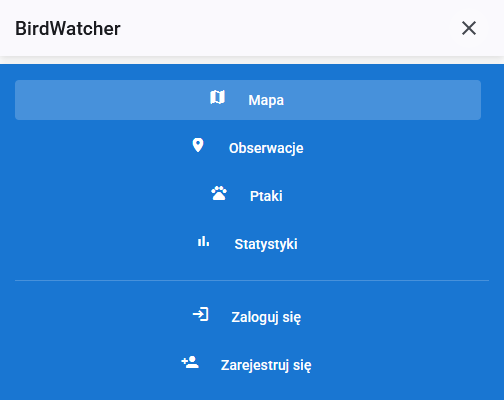
\includegraphics[width=0.6\textwidth]{/chapter4/navbar2.png}
	\caption{Pasek nawigacyjny w trybie rozwijanym}
	\label{fig:navbar2}
\end{figure}

\subsubsection{Strona główna}
Strona główna zawiera interaktywną mapę wyświetlająca obserwację zaznaczone pinezkami z podziałem na tygodnie w roku.

\begin{figure}[!htb]
	\centering
	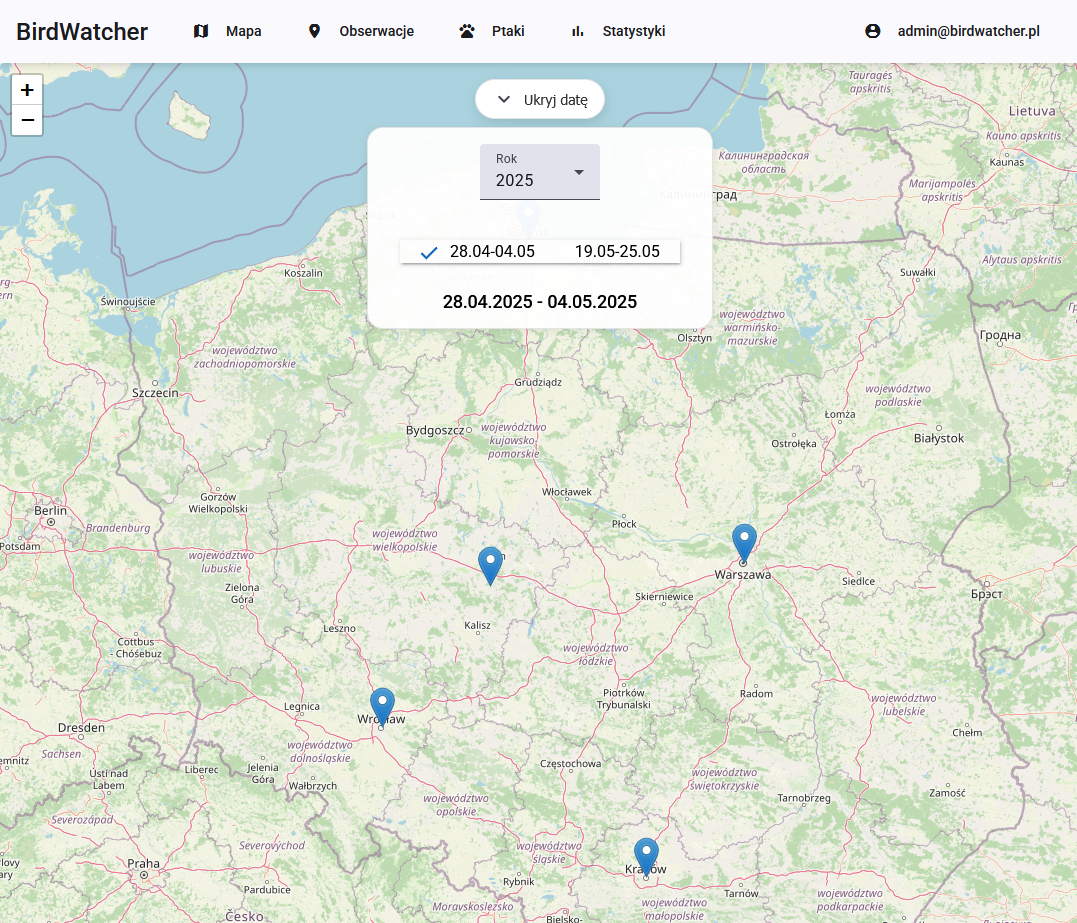
\includegraphics[width=0.6\textwidth]{/chapter4/mainpage1.png}
	\caption{Strona główna z mapą interaktywną}
	\label{fig:mainpage1}
\end{figure}

\subsubsection{Komponenty ptaków}
Zaimplementowane zostały następujące komponenty ptaków:
\begin{itemize}
	\item Lista ptaków
	\item Formularz dodawania oraz edycji ptaków
	\item Strona szczegółów ptaka
\end{itemize}

\begin{figure}[!htb]
	\centering
	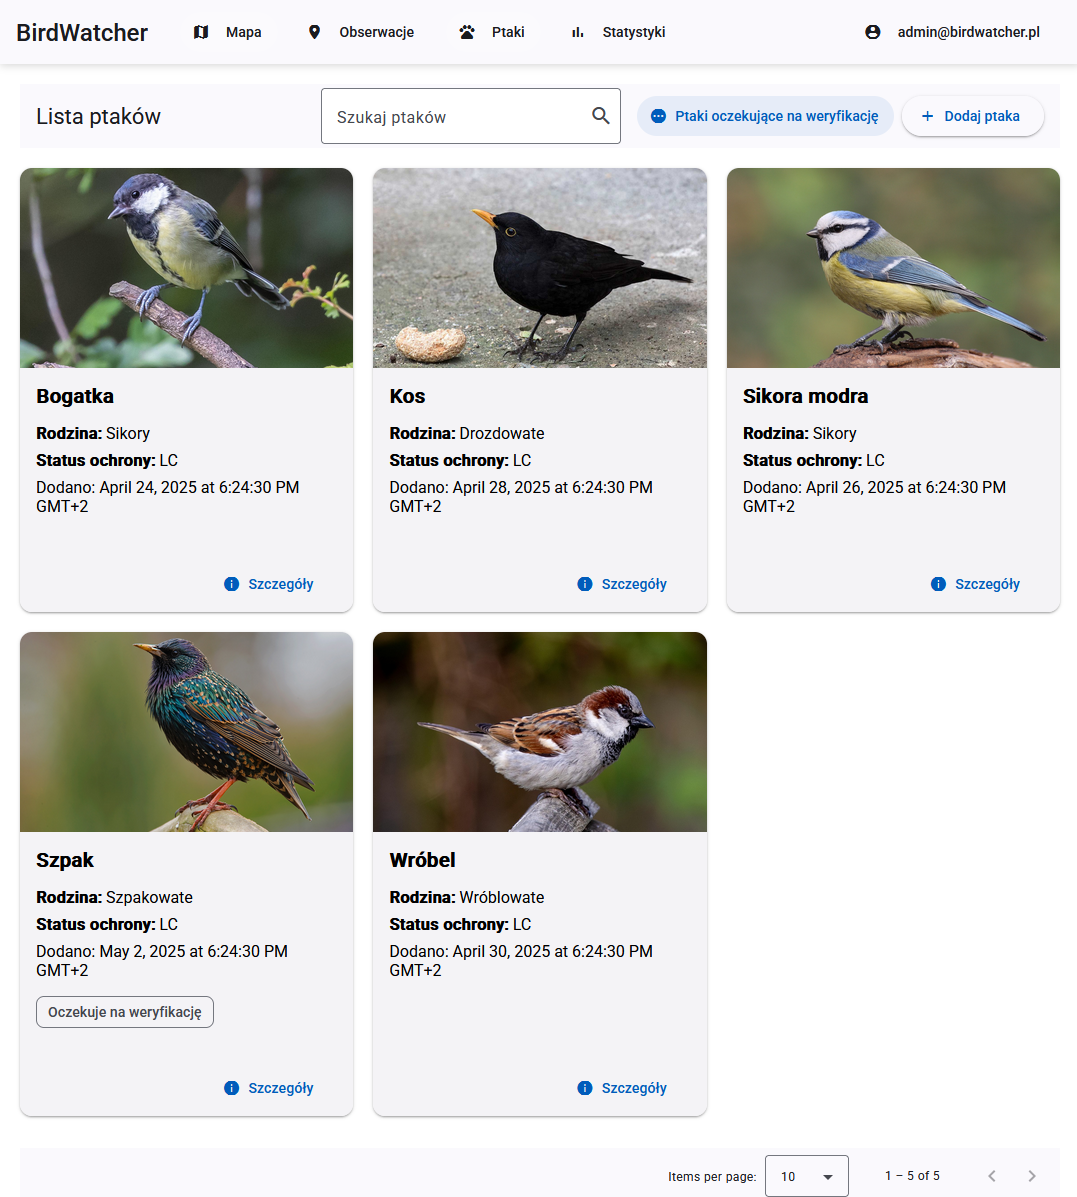
\includegraphics[width=0.6\textwidth]{/chapter4/ptaki1.png}
	\caption{Strona listy ptaków}
	\label{fig:ptaki1}
\end{figure}

\begin{figure}[!htb]
	\centering
	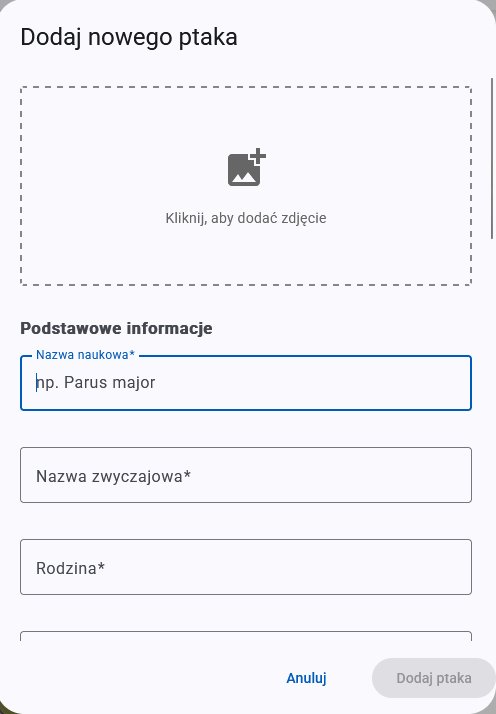
\includegraphics[width=0.4\textwidth]{/chapter4/ptaki2.png}
	\caption{Formularz dodawania/edycji ptaka}
	\label{fig:ptaki2}
\end{figure}

\begin{figure}[!htb]
	\centering
	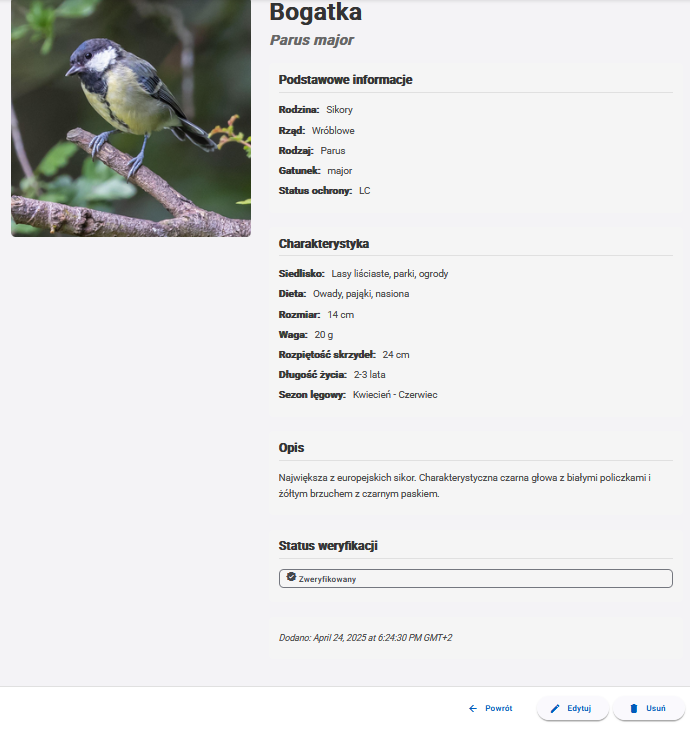
\includegraphics[width=0.6\textwidth]{/chapter4/ptaki3.png}
	\caption{Strona szczegółów ptaka}
	\label{fig:ptaki3}
\end{figure}

\subsubsection{Komponenty obserwacji}
Zaimplementowane zostały następujące komponenty związane z obserwacjami:
\begin{itemize}
	\item Lista obserwacji ptaków
	\item Formularz dodawania oraz edycji obserwacji
	\item Strona szczegółów obserwacji wraz z galerią obrazów
\end{itemize}

\begin{figure}[!hb]
	\centering
	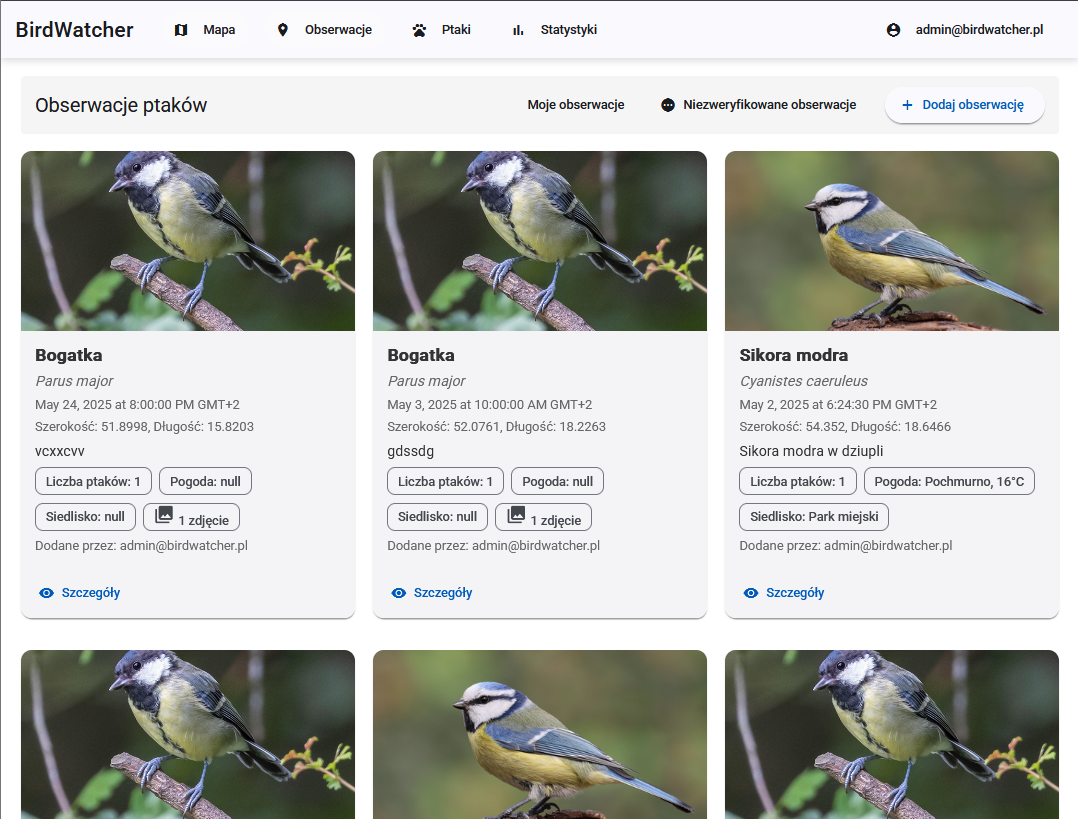
\includegraphics[width=0.6\textwidth]{/chapter4/obserwacje1.png}
	\caption{Strona listy obserwacji}
	\label{fig:obserwacje1}
\end{figure}

\begin{figure}[!hb]
	\centering
	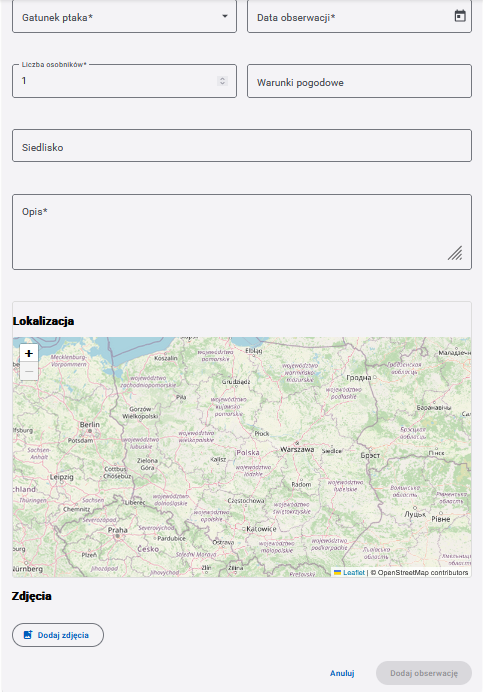
\includegraphics[width=0.4\textwidth]{/chapter4/obserwacje2.png}
	\caption{Formularz dodawania/edycji obserwacji}
	\label{fig:obserwacje2}
\end{figure}

\begin{figure}[!htb]
	\centering
	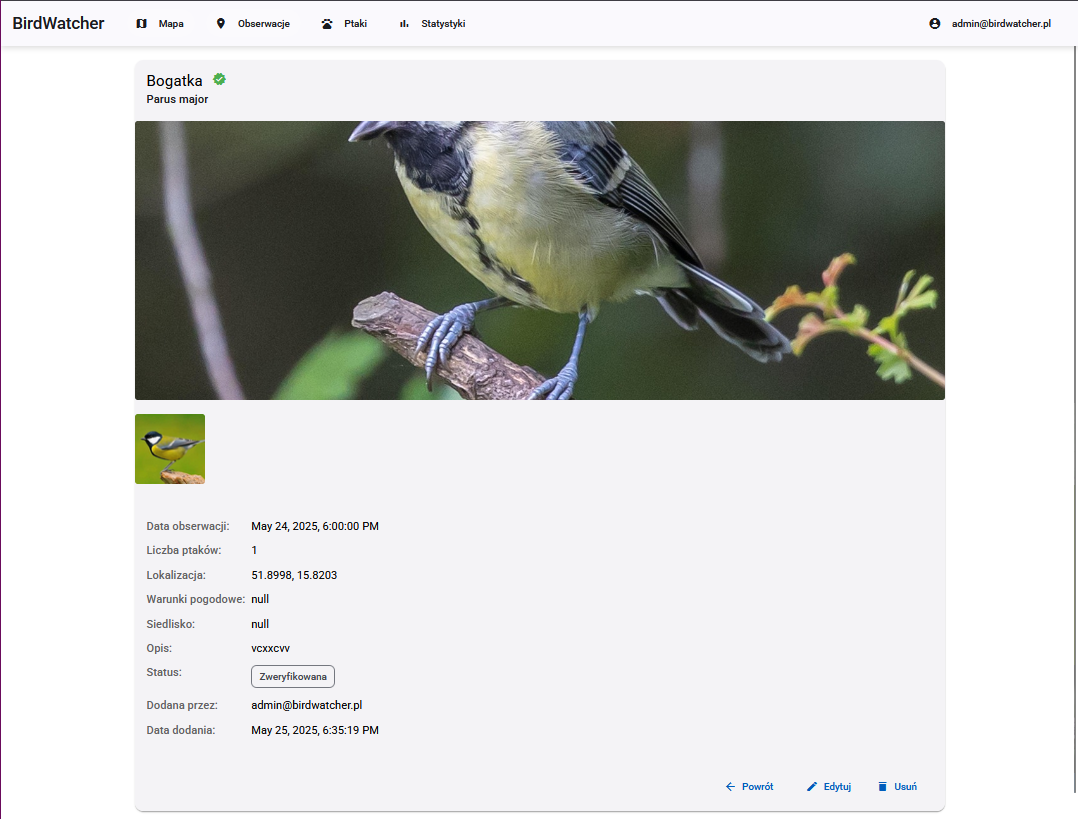
\includegraphics[width=0.6\textwidth]{/chapter4/obserwacje3.png}
	\caption{Strona szczegółów obserwacji}
	\label{fig:obserwacje3}
\end{figure}

\subsubsection{Komponenty użytkownika}
Zaimplementowane zostały następujące komponenty związane z użytkownikami:
\begin{itemize}
	\item Formularz logowania
	\item Formularz rejestracji
	\item Formularz zmiany danych użytkownika
\end{itemize}

\begin{figure}[!htb]
	\centering
	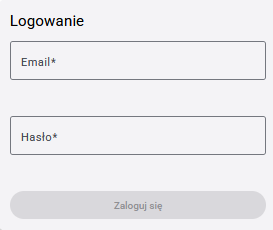
\includegraphics[width=0.6\textwidth]{/chapter4/logowanie.png}
	\caption{Formularz logowania}
	\label{figlogowanie}
\end{figure}

\begin{figure}[!htb]
	\centering
	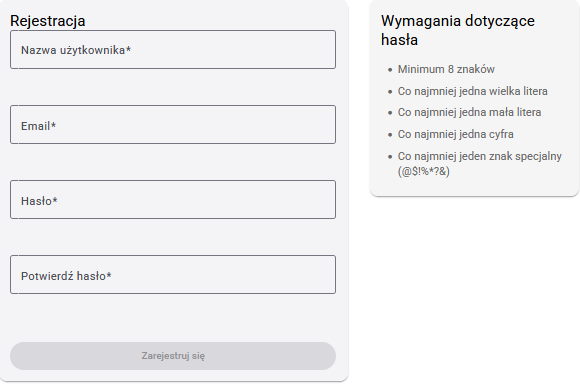
\includegraphics[width=0.6\textwidth]{/chapter4/rejestracja.png}
	\caption{Formularz rejestracji}
	\label{fig:rejestracja}
\end{figure}

\begin{figure}[!htb]
	\centering
	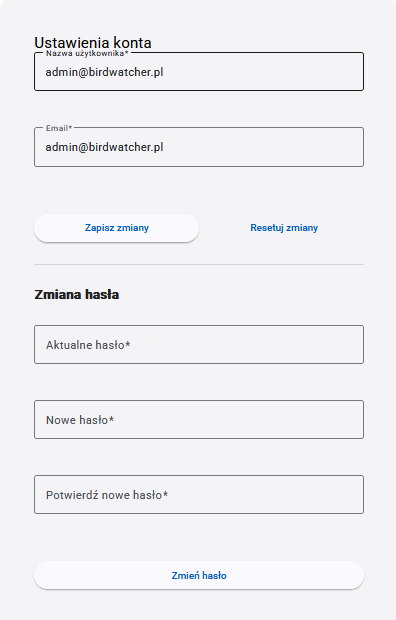
\includegraphics[width=0.6\textwidth]{/chapter4/konto.png}
	\caption{Formularz konta użytkownika}
	\label{fig:konto}
\end{figure}

\subsection{Podsumowanie implementacji frontendu}
\index{Podsumowanie implementacji frontendu}

Aplikacja frontendowa wykonana w technologii Angular została stworzona zgodnie z przyjętymi koncepcjami Angular oraz praktykując najlepsze techniki programowania obiektowego i wzorcami projektowymi. Wykorzystanie komponentów Material znacznie przyśpieszyło pracę nad systemem oraz zapewniło spójny wygląd aplikacji. Strona jest responsywna, dostosowuje się do różnych rozmiarów ekranów i ma przejrzysty interfejs. Dzięki zastosowaniu REST API, gdzie większość wymagających operacji na danyc odbywa się na backendzie i wykorzystaniu techniki paginacji aplikacja działa szybko i nie wymaga dużych zasobów mocy do działania po stronie klienta.

\FloatBarrier

\section{Implementacja backendu}
\index{Implementacja backendu}

\subsection{Architektura aplikacji backendowej}
\index{Architektura aplikacji backendowej}
Backend został stworzony przy użyciu frameworka ASP.NET Core 8.0. W aplikacji wykorzystane zostały wzorce projektowe Repository Pattern oraz Dependency Injection. REST Api zostało zaprojektowane zgodnie ze standardami co zapewnia spójny interfejs komunikacji z frontendem. Podejście projektowania bazy danych opiera się na Code First - najpierw tworzy się modele danych w kodzie a następnie na ich podstawię tworzone są migrację bazy danych zawierające odpowiednie polecenia SQL do tworzenia struktury.

\subsection{Konfiguracja aplikacji}
\index{Konfiguracja aplikacji}

Główna aplikacja znajduje się w pliku Program.cs, w którym zostały skonfigurowane niezbędne komponenty dotyczące kontrolerów API, serwisów, bazy danych, bezpieczeństwa i autoryzacji.

\begin{lstlisting}[style=csharp, caption={Fragment pliku Program.cs}]
var builder = WebApplication.CreateBuilder(args);
[...]
// Add services to the container.
builder.Services.AddControllers();
builder.Services.AddEndpointsApiExplorer();
builder.Services.AddSwaggerGen();
// Add DbContext
builder.Services.AddDbContext<ApplicationDbContext>(
	options =>options.UseSqlite(builder.Configuration
		.GetConnectionString("DefaultConnection")));
// Add Identity
builder.Services.AddIdentity<ApplicationUser, IdentityRole>(options =>
{
	// Password settings[...]
	// Lockout settings[...]
	// User settings[...]
})
.AddEntityFrameworkStores<ApplicationDbContext>()
.AddDefaultTokenProviders();
// Add Authorization Policies
builder.Services.AddAuthorization(options =>
{
	options.AddPolicy("RequireAdminRole", policy =>
	policy.RequireRole(AuthorizationConstants.AdminRole));
	options.AddPolicy("RequireUserRole", policy =>
	policy.RequireRole(AuthorizationConstants.UserRole));
});
// Add CORS
builder.Services.AddCors(options => [...]
// Add Authentication
var jwtKey = builder.Configuration["Jwt:Key"];[...]
builder.Services.AddAuthentication(options =>[...]
.AddJwtBearer(options =>[...]
// Add Services
builder.Services.AddScoped<IAuthService, AuthService>();
builder.Services.AddScoped<IBirdService, BirdService>();
builder.Services.AddScoped<IBirdObservationService, BirdObservationService>();
var app = builder.Build();
// Automatyczne tworzenie bazy danych i inicjalizacja danych
[...]
// Configure the HTTP request pipeline.
if (app.Environment.IsDevelopment())
{
	app.UseSwagger();
	app.UseSwaggerUI();
}
[...]
app.UseHttpsRedirection();
app.UseStaticFiles(); // Dodaj obsługę statycznych plików
app.UseCors("AllowAngularDevServer");
app.UseAuthentication();
app.UseAuthorization();
app.MapControllers();
app.Run();
\end{lstlisting}

\subsection{Model danych}
\index{Model danych}

\subsubsection{Kontekst bazy danych}
System wykorzystuje ORM Entity Framework Core z bazą danych SQLite. Kontekst bazy danych \texttt{ApplicationDbContext} dziedziczy po \texttt{IdentityDbContext<ApplicationUser>} co umożliwia integrację z systemem autoryzacji ASP.NET Core Identity.

\begin{lstlisting}[style=csharp, caption={Implementacja ApplicationDbContext}]
namespace BackendService.Data
{
	public class ApplicationDbContext : IdentityDbContext<ApplicationUser>
	{
		public ApplicationDbContext(DbContextOptions
		<ApplicationDbContext> options)
		: base(options)
		{}
		
		public DbSet<Bird> Birds { get; set; }
		public DbSet<BirdObservation> BirdObservations { get; set; }
		
		protected override void OnModelCreating(ModelBuilder modelBuilder)
		{
			base.OnModelCreating(modelBuilder);
			
			modelBuilder.Entity<Bird>()
			.HasOne<ApplicationUser>()
			.WithMany()
			.HasForeignKey(b => b.UserId)
			.OnDelete(DeleteBehavior.Restrict);
			
			modelBuilder.Entity<BirdObservation>()
			.HasOne(b => b.Bird)
			.WithMany(b => b.Observations)
			.HasForeignKey(b => b.BirdId)
			.OnDelete(DeleteBehavior.Cascade);
		}
	}
}
\end{lstlisting}

\subsubsection{Modele domenowe}
Aplikacja zawiera kilka klas zawierających modele domenowe:
\begin{itemize}
	\item \texttt{ApplicationUser} - rozszerzony model użytkownika z ASP.NET Core Identity
	\item \texttt{Bird} - model danych ptaka
	\item \texttt{BirdObservation} - model danych obserwacji
\end{itemize}

\begin{lstlisting}[style=csharp, caption={Implementacja ApplicationUser}]
public class ApplicationUser : IdentityUser
{
	public string? RefreshToken { get; set; }
	public DateTime? RefreshTokenExpiryTime { get; set; }
	public DateTime CreatedAt { get; set; } = DateTime.UtcNow;
	public ICollection<Bird> Birds { get; set; } = new List<Bird>();
	public ICollection<BirdObservation> BirdObservations { get; set; } = new List<BirdObservation>();
}
\end{lstlisting}

\begin{lstlisting}[style=csharp, caption={Fragment implementacji Bird}]
public class Bird
{
	public int Id { get; set; }
	
	[Required]
	public string CommonName { get; set; } = string.Empty;
	
	[Required]
	public string ScientificName { get; set; } = string.Empty;
	
	[Required]
	public string Family { get; set; } = string.Empty;
	
	public string? Order { get; set; }
	public string? Genus { get; set; }
	public string? Species { get; set; }
...
\end{lstlisting}

\begin{lstlisting}[style=csharp, caption={Fragment implementacji BirdObservation}]
public class BirdObservation
{
	public int Id { get; set; }
	
	[Required]
	public int BirdId { get; set; }
	public Bird Bird { get; set; } = null!;
	
	[Required]
	public string UserId { get; set; } = string.Empty;
	public ApplicationUser User { get; set; } = null!;
	
	[Required]
	public double Latitude { get; set; }
...
\end{lstlisting}

\subsection{Kontrolery API}
\index{Kontrolery API}

Architektura kontrolerów została zaprojektowana zgodnie z wzorcem REST API - każdy kontroler odpowiada za konkretną część domeny biznesowej. Wszystkie kontrolery dziedziczą po \texttt{ControllerBase} i są oznaczone atrybutami \texttt{[ApiController]} oraz \texttt{[Route("api/[controller]")]} co w ASP.NET Core automatycznie generuje ścieżki API na podstawie nazw kontrolerów oraz metod.

\begin{lstlisting}[style=csharp, caption={Fragment implementacji BirdsObervationsController}]
namespace BackendService.Controllers
{
	[ApiController]
	[Route("api/[controller]")]
	public class BirdObservationsController : ControllerBase
	{
		private readonly IBirdObservationService _observationService;
		
		public BirdObservationsController(IBirdObservationService observationService)
		{
			_observationService = observationService;
		}
		
		[HttpGet]
		public async Task<ActionResult<PaginatedResponse<
			BirdObservationDto>>> GetObservations([FromQuery] PaginationParams paginationParams)
		{
			var observations = await _observationService.GetAllObservationsAsync(
				paginationParams);
			return Ok(observations);
		}
		
		[HttpGet("user")]
		[Authorize]
		public async Task<ActionResult<PaginatedResponse<
			BirdObservationDto>>> GetUserObservations([FromQuery] PaginationParams paginationParams)
		{
			var userId = User.FindFirst(ClaimTypes.NameIdentifier)?.Value;
			if (string.IsNullOrEmpty(userId))
			{
				return Unauthorized();
			}
			
			var observations = await _observationService.GetUserObservationsAsync(
				userId, paginationParams);
			return Ok(observations);
		}
...
\end{lstlisting}

\subsection{Warstwa serwisów}
\index{Warstwa serwisów}
System wykorzystuje wzorzec \texttt{Dependency Injection} do zarządzania zależnościami. Serwisy są rejestrowane w \texttt{kontenerze DI} w pliku \texttt{Program.cs}

\begin{lstlisting}[style=csharp, caption={Fragment Program.cs z rejestrowaniem serwisów}]
builder.Services.AddScoped<IAuthService, AuthService>();
builder.Services.AddScoped<IBirdService, BirdService>();
builder.Services.AddScoped<IBirdObservationService, BirdObservationService>();
\end{lstlisting}

\subsection{Obsługa plików}
\index{Obsługa plików}
Aplikacja obsługuje przesyłanie i zapisywanie na backendzie plików graficznych. Pliki te są elementami ptaków oraz obserwacji. Pliki zapisywane są w katalogu \texttt{wwwroot/uploads} z unikalnymi nazwami generowanymi na podstawię \texttt{GUID} i są widoczne z poziomu aplikacji frontendowej.

\begin{lstlisting}[style=csharp, caption={Fragment implementacji zapisu plików}]
private async Task<string> SaveImageAsync(IFormFile image)
{
	var uniqueFileName = $"{Guid.NewGuid()}_{image.FileName}";
	var filePath = Path.Combine(_uploadFolder, uniqueFileName);
	
	using (var fileStream = new FileStream(filePath, FileMode.Create))
	{
		await image.CopyToAsync(fileStream);
	}
	
	return $"/uploads/birds/{uniqueFileName}";
}
\end{lstlisting}

\subsection{Walidacja danych}
\index{Walidacja danych}
Modele danych wykorzystują \texttt{[Data Adnnotations]} do walidacji prawidłowości danych po stronie serwisów.

\begin{lstlisting}[style=csharp, caption={Przykład stosowania adnotacji w modelu DTO}]
public class CreateBirdDto
{
	[Required]
	public string CommonName { get; set; } = string.Empty;
	
	[Required]
	public string ScientificName { get; set; } = string.Empty;
	
	[Required]
	public string Family { get; set; } = string.Empty;
	
	[Required]
	public string ConservationStatus { get; set; } = string.Empty;
	
	[Required]
	[MaxLength(1000)]
	public string Description { get; set; } = string.Empty;
	
	public IFormFile? Image { get; set; }
}
\end{lstlisting}

\subsection{Paginacja}
\index{Paginacja}
Aplikacja wykorzystuje dzielenie danych na mniejsze zbiory podczas prezentowania list. Zapewnia to wysoką wydajność aplikacji frontendowej oraz szybkie przesyłanie danych w mniejszych porcjach w przypadku dużych zbiorów.

\begin{lstlisting}[style=csharp, caption={Implementacja paginacji po stronie backendu}]
public class PaginationParams
{
	private const int MaxPageSize = 50;
	private int _pageSize = 10;
	
	public int PageNumber { get; set; } = 1;
	public int PageSize
	{
		get => _pageSize;
		set => _pageSize = value > MaxPageSize ? MaxPageSize : value;
	}
}

public class PaginatedResponse<T>
{
	public IEnumerable<T> Items { get; set; } = new List<T>();
	public int TotalCount { get; set; }
	public int PageNumber { get; set; }
	public int PageSize { get; set; }
	public int TotalPages { get; set; }
	public bool HasPreviousPage { get; set; }
	public bool HasNextPage { get; set; }
}
\end{lstlisting}

\subsection{Obsługa błędów}
\index{Obsługa błędów}
System implementuje globalną obsługę wyjątków poprzez wykorzystanie \texttt{middleware} oraz zwracanie odpowiednich kodów \texttt{HTTP} zgodnie z obowiązującymi standardami.

\begin{lstlisting}[style=csharp, caption={Przykład obsługi błędów w kontrolerze}]
[HttpPut("{id}")]
[Authorize(Roles = AuthorizationConstants.AdminRole)]
public async Task<IActionResult> UpdateBird(int id, [FromForm] UpdateBirdDto birdDto)
{
	try
	{
		await _birdService.UpdateBirdAsync(id, birdDto);
		return NoContent();
	}
	catch (KeyNotFoundException)
	{
		return NotFound();
	}
	catch (UnauthorizedAccessException)
	{
		return Forbid();
	}
}
\end{lstlisting}

\subsection{Konfiguracja CORS}
CORS zostały odpowiednio skonfigurowane w pliku \texttt{Program.cs} aby umożliwić obsługę żądań aplikacji frontendowej Angular.

\begin{lstlisting}[style=csharp, caption={Konfiguracja CORS}]
builder.Services.AddCors(options =>
{
	options.AddPolicy("AllowAngularDevServer",
	builder => builder
	.WithOrigins("http://localhost:4200", "https://localhost:4200")
	.AllowAnyMethod()
	.AllowAnyHeader()
	.WithExposedHeaders("Token-Expired")
	.AllowCredentials());
});
\end{lstlisting}

\subsection{Interfejs Swagger}
\index{Interfejs Swagger}
Lista \texttt{endpointów} oraz struktur wykorzystywanych w REST API jest przedstawiona w interfejsie Swagger zawartym w dodatku \ref{chapter:dodatek_A}. Dzięki interfejsowi Swagger z łatwością testuje się implementowane API oraz ułatwia on implementacje komunikacji po stronie frontendu.

\subsection{Podsumowanie implementacji backendu}
\index{Podsumowanie implementacji backendu}
Część backendowa aplikacji została zaprojektowana zgodnie z obowiązującymi najlepszymi praktykami programowania, wzorcami projektowymi oraz zaleceniami Microsoftu. Stworzony system jest modularny, łatwy w rozwoju, wydajny i bezpieczny dzięki wykorzystaniu \texttt{ASP.NET Core} w połączeniu z \texttt{Entity Framework Core}. Architektura REST API zapewnia efektywną komunikację, a implementacja paginacji wydajność ładowania danych i oszczędność zasobów.

\section{Implementacja bazy danych}
\index{Implementacja bazy danych}
Baza danych w systemie została zaimplementowana z użyciem \texttt{SQLite3} oraz \texttt{Entity Framework Core} wykorzystując podejście \texttt{code first}.

\subsection{Konfiguracja połączenia z bazą danych}
\index{Konfiguracja połączenia z bazą danych}
Połączenie z bazą danych zostało skonfigurowane w pliku \texttt{appsettings.json}

\begin{lstlisting}[style=csharp, caption={Konfiguracja bazy w appsettings.json}]
{
	"ConnectionStrings": {
		"DefaultConnection": "Data Source=birdwatcher.db"
	}
}
\end{lstlisting}

Plik bazy danych \texttt{birdwatcher.db} jest automatycznie tworzony przy pierwszym starcie aplikacji oraz automatycznie aktualizowany gdy powstają nowe migracje.

\subsection{Struktura bazy danych}
\index{Struktura bazy danych}

\subsubsection{Tabela AspNetUsers (Identity)}
Tabela \texttt{AspNetUsers} jest częścią systemu \texttt{ASP.NET Core Identity}, została rozszerzona o dodatkowe pola potrzebne w systemie i służy ona do przechowywania danych o użytkownikach.

\begin{lstlisting}[style=sqlstyle, caption={Struktura tabeli AspNetUsers}]
CREATE TABLE AspNetUsers (
	Id TEXT PRIMARY KEY,
	UserName TEXT,
	NormalizedUserName TEXT,
	Email TEXT,
	NormalizedEmail TEXT,
	EmailConfirmed INTEGER,
	PasswordHash TEXT,
	SecurityStamp TEXT,
	ConcurrencyStamp TEXT,
	PhoneNumber TEXT,
	PhoneNumberConfirmed INTEGER,
	TwoFactorEnabled INTEGER,
	LockoutEnd TEXT,
	LockoutEnabled INTEGER,
	AccessFailedCount INTEGER,
	RefreshToken TEXT,
	RefreshTokenExpiryTime TEXT,
	CreatedAt TEXT NOT NULL
);
\end{lstlisting}

\subsubsection{Tabela AspNetRoles (Identity)}
Tabela \texttt{AspNetRoles} przechowuje informację o rolach użytkowników.

\begin{lstlisting}[style=sqlstyle, caption={Struktura tabeli AspNetRoles}]
CREATE TABLE AspNetRoles (
	Id TEXT PRIMARY KEY,
	Name TEXT,
	NormalizedName TEXT,
	ConcurrencyStamp TEXT
);
\end{lstlisting}

\subsubsection{Tabela AspNetUserRoles (Identity)}
Tabela \texttt{AspNetUserRoles} łaczy użytkowników z rolami.

\begin{lstlisting}[style=sqlstyle, caption={Struktura tabeli AspNetRoles}]
CREATE TABLE AspNetUserRoles (
	UserId TEXT NOT NULL,
	RoleId TEXT NOT NULL,
	PRIMARY KEY (UserId, RoleId),
	FOREIGN KEY (UserId) REFERENCES AspNetUsers(Id) ON DELETE CASCADE,
	FOREIGN KEY (RoleId) REFERENCES AspNetRoles(Id) ON DELETE CASCADE
);
\end{lstlisting}

\subsubsection{Tabela Birds}
Tabela \texttt{Birds} przechowuje informację o ptakach.

\begin{lstlisting}[style=sqlstyle, caption={Struktura tabeli AspNetRoles}]
CREATE TABLE Birds (
	Id INTEGER PRIMARY KEY AUTOINCREMENT,
	CommonName TEXT NOT NULL,
	ScientificName TEXT NOT NULL,
	Family TEXT NOT NULL,
	Order TEXT,
	Genus TEXT,
	Species TEXT,
	ConservationStatus TEXT NOT NULL,
	Description TEXT NOT NULL,
	Habitat TEXT,
	Diet TEXT,
	Size TEXT,
	Weight REAL,
	Wingspan REAL,
	Lifespan TEXT,
	BreedingSeason TEXT,
	ImageUrl TEXT,
	IsVerified INTEGER NOT NULL DEFAULT 0,
	UserId TEXT NOT NULL,
	CreatedAt TEXT NOT NULL,
	FOREIGN KEY (UserId) REFERENCES AspNetUsers(Id) ON DELETE RESTRICT
);
\end{lstlisting}

\subsubsection{Tabela BirdObervations}
Tabela \texttt{BirdObersvations} przechowuje informację o obserwacjach ptaków.

\begin{lstlisting}[style=sqlstyle, caption={Struktura tabeli AspNetRoles}]
CREATE TABLE BirdObservations (
	Id INTEGER PRIMARY KEY AUTOINCREMENT,
	BirdId INTEGER NOT NULL,
	UserId TEXT NOT NULL,
	Latitude REAL NOT NULL,
	Longitude REAL NOT NULL,
	ObservationDate TEXT NOT NULL,
	Description TEXT,
	NumberOfBirds INTEGER,
	WeatherConditions TEXT,
	Habitat TEXT,
	IsVerified INTEGER NOT NULL DEFAULT 0,
	CreatedAt TEXT NOT NULL,
	UpdatedAt TEXT NOT NULL,
	ImageUrls TEXT NOT NULL DEFAULT '[]',
	FOREIGN KEY (BirdId) REFERENCES Birds(Id) ON DELETE CASCADE,
	FOREIGN KEY (UserId) REFERENCES AspNetUsers(Id) ON DELETE CASCADE
);
\end{lstlisting}

\newpage

\subsection{Relacje}
\index{Relacje}

\subsubsection{Diagram relacji}

\begin{figure}[!htb]
	\centering
	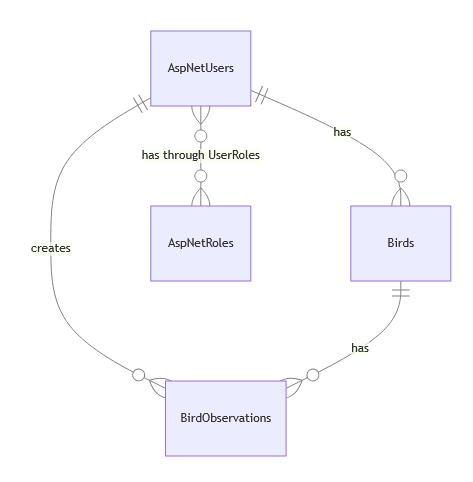
\includegraphics[width=0.6\textwidth]{/chapter4/diagramrelacji.png}
	\caption{Uproszczony diagram relacji bazy danych}
	\label{fig:diagramrelacji}
\end{figure}

\subsubsection{Konfiguracja relacji w Entity Framework Core}

\begin{lstlisting}[style=csharp, caption={Konfiguracja relacji w Entity Framework Core}]
protected override void OnModelCreating(ModelBuilder modelBuilder)
{
	base.OnModelCreating(modelBuilder);
	
	modelBuilder.Entity<Bird>()
	.HasOne<ApplicationUser>()
	.WithMany()
	.HasForeignKey(b => b.UserId)
	.OnDelete(DeleteBehavior.Restrict);
	
	modelBuilder.Entity<BirdObservation>()
	.HasOne(b => b.Bird)
	.WithMany(b => b.Observations)
	.HasForeignKey(b => b.BirdId)
	.OnDelete(DeleteBehavior.Cascade);
}
\end{lstlisting}

\subsection{Indeksy bazy danych}
\index{Indeksy bazy danych}
W bazie danych zostały utworzone następujące indeksy aby poprawić wydajność wyszukiwania.

\begin{lstlisting}[style=sqlstyle, caption={Indeksy bazy danych}]
-- Indeksy dla tabeli Birds
CREATE INDEX IX_Birds_CommonName ON Birds(CommonName);
CREATE INDEX IX_Birds_ScientificName ON Birds(ScientificName);

-- Indeksy dla tabeli BirdObservations
CREATE INDEX IX_BirdObservations_BirdId ON BirdObservations(BirdId);
CREATE INDEX IX_BirdObservations_UserId ON BirdObservations(UserId);
CREATE INDEX IX_BirdObservations_ObservationDate ON BirdObservations(ObservationDate);
CREATE INDEX IX_BirdObservations_Latitude_Longitude ON BirdObservations(Latitude, Longitude);

-- Indeksy dla tabeli AspNetUsers (Identity)
CREATE INDEX IX_AspNetUsers_Email ON AspNetUsers(Email);
CREATE INDEX IX_AspNetUsers_UserName ON AspNetUsers(UserName);
\end{lstlisting}

\subsection{Migracje}
\index{Migracje}
W aplikacji wykorzystywany jest \texttt{Code-First Migrations Entity Framework Core} do zarządzania schematem bazy danych.
Historia migracji jest przechowywana w osobnych plikach nazwanych opisowo np.:
\begin{enumerate}
	\item InitalCreate
	\item AddBirdsAndObserwations
	\item AddRefreshToken
	\item ...
\end{enumerate}

\subsection{Backup i odzyskiwanie}
\index{Backup i odzyskiwanie}
Ponieważ SQLite przechowuje bazę danych jako jeden plik na dysku, backup sprowadza się do skopiowania pliku \texttt{birdwatcher.db}

\begin{lstlisting}[language=bash, caption={Przykład skryptu kopiującego w bash}]
cp birdwatcher.db backup/birdwatcher_$(date +%Y%m%d_%H%M%S).db
\end{lstlisting}

\subsection{Automatyczne tworzenie bazy danych}
\index{Automatyczne tworzenie bazy danych}
Automatyczne tworzenie bazy danych zostało zaimplementowane w pliku \texttt{Program.cs}.

\begin{lstlisting}[style=csharp, caption={Automatyczne tworzenie bazy danych}]
using (var scope = app.Services.CreateScope())
	{
		var services = scope.ServiceProvider;
		try
		{
			var context = services.GetRequiredService
			<ApplicationDbContext>();
			context.Database.EnsureCreated();
			await SeedData.Initialize(services);
		}
		catch (Exception ex)
		{
			var logger = services.GetRequiredService<ILogger<Program>>();
			logger.LogError(ex, "Wystąpił błąd podczas tworzenia bazy danych.");
		}
	}
\end{lstlisting}

\subsection{Podsumowanie implementacji bazy danych}
\index{Podsumowanie implementacji bazy danych}

\FloatBarrier

\section{Implementacja systemu autentyfikacji i autoryzacji}
\index{Implementacja systemu autentyfikacji i autoryzacji}

\section{Implementacja funkcjonalności mapy i geolokalizacji}
\index{Implementacja funkcjonalności mapy i geolokalizacji} % chapter4.tex zawiera treść rozdziału 4

%----------------------------------------------------------------------------------------
%	ROZDZIAŁ 5
%----------------------------------------------------------------------------------------
%%%%%%%%%%%%%%%%%%%%%%%%%%%%%%%%%%%%%%%%%
% Szablon pracy dyplomowej
% Wydział Informatyki 
% Zachodniopomorski Uniwersytet Technologiczny w Szczecinie
% autor Joanna Kołodziejczyk (jkolodziejczyk@zut.edu.pl)
% Bardzo wczesnym pierwowzorem szablonu był
% The Legrand Orange Book
% Version 5.0 (29/05/2025)
%
% Modifications to LOB assigned by %JK
%%%%%%%%%%%%%%%%%%%%%%%%%%%%%%%%%%%%%%%%%


%----------------------------------------------------------------------------------------
%	CHAPTER 5
%----------------------------------------------------------------------------------------
\sloppy

\chapter{Testy}
\label{rozdzial5} % chapter5.tex zawiera treść rozdziału 5

%----------------------------------------------------------------------------------------
%	ROZDZIAŁy kolejne należy dodać analogicznie do 1 i 2 
% utworzyć pliki i je załączyć (include)
%----------------------------------------------------------------------------------------

%----------------------------------------------------------------------------------------
%	ZAKOŃCZENIE PRACY DYPLOMOWEJ (JK - design and implementation)
%----------------------------------------------------------------------------------------
\addcontentsline{toc}{chapter}{Podsumowanie}
%%%%%%%%%%%%%%%%%%%%%%%%%%%%%%%%%%%%%%%%%
% Wnioski do pracy dyplomowej
% Szablon pracy dyplomowej
% Wydział Informatyki 
% Zachodniopomorski Uniwersytet Technologiczny w Szczecinie
% autor Joanna Kołodziejczyk (jkolodziejczyk@zut.edu.pl)
% Bardzo wczesnym pierwowzorem szablonu był
% The Legrand Orange Book
% Version 5.0 (29/05/2025)
%
% Modifications to LOB assigned by %JK
%%%%%%%%%%%%%%%%%%%%%%%%%%%%%%%%%%%%%%%%%


\chapter*{Podsumowanie}

Podsumowanie pracy powinno na maksymalnie dwóch stronach przedstawić główne wyniki pracy dyplomowej. Struktura zakończenia to:
\begin{enumerate}
\item Przypomnienie celu i hipotez
\item Co w pracy wykonano by cel osiągnąć (analiza, projekt, oprogramowanie, badania eksperymentalne)
\item Omówienie głównych wyników pracy
\item Jak wyniki wzbogacają dziedzinę
\item Zamknięcie np. poprzez wskazanie dalszych kierunków badań.
\end{enumerate} % conclusions.tex zawiera treść zakończenia/podsumowania pracy dyplomowej


%----------------------------------------------------------------------------------------
%	SPIS LITERATURY (JK - design and implementation)
%----------------------------------------------------------------------------------------
\pagestyle{empty} 
\chapter*{Spis literatury}
\addcontentsline{toc}{chapter}{\textcolor{blueZUT}{Spis literatury}}
% Poniżej zdefiniowane są filtry do dzielenia spisu literatury na kategorie
\defbibfilter{articles}{
  type=article or 
  type=inproceedings
}
\defbibfilter{other}{
  type=url or
  type=online  or
  type=manual or
  type=misc
}

% UWAGA! -aby zmienić zawartość spisu literatury należy wyedytować plik
% bibliography.bib

%------------------------------------------------
% Spis literartury podzielony jest na 3 kategorie
% 1
\section*{Książki}
\addcontentsline{toc}{section}{Książki}
\printbibliography[heading=bibempty,type=book]

%------------------------------------------------
% 2
\section*{Artykuły}
\addcontentsline{toc}{section}{Artykuły}
\printbibliography[heading=bibempty,filter=articles]
%------------------------------------------------
% 3
\section*{Źródła internetowe i inne}
\addcontentsline{toc}{section}{Źródła internetowe i inne}
\printbibliography[heading=bibempty,filter=other]


%----------------------------------------------------------------------------------------
%	APPENDIX (JK - design and implementation)
%----------------------------------------------------------------------------------------
\pagestyle{fancy} 
\begin{appendix}
\appendix
%%%%%%%%%%%%%%%%%%%%%%%%%%%%%%%%%%%%%%%%%
% Szablon pracy dyplomowej
% Wydział Informatyki 
% Zachodniopomorski Uniwersytet Technologiczny w Szczecinie
% autor Joanna Kołodziejczyk (jkolodziejczyk@zut.edu.pl)
% Bardzo wczesnym pierwowzorem szablonu był
% The Legrand Orange Book
% Version 5.0 (29/05/2025)2023)
%
% Modifications to LOB assigned by %JK
%%%%%%%%%%%%%%%%%%%%%%%%%%%%%%%%%%%%%%%%%
\thispagestyle{empty}
\listoffigures

\chapter{Swagger}
\label{chapter:dodatek_A}

\textit{Poniżej przedstawiono interfejs Swagger prezentujący dostępne endpointy API oraz struktury danych.}

\begin{figure}[!htb]
	\centering
	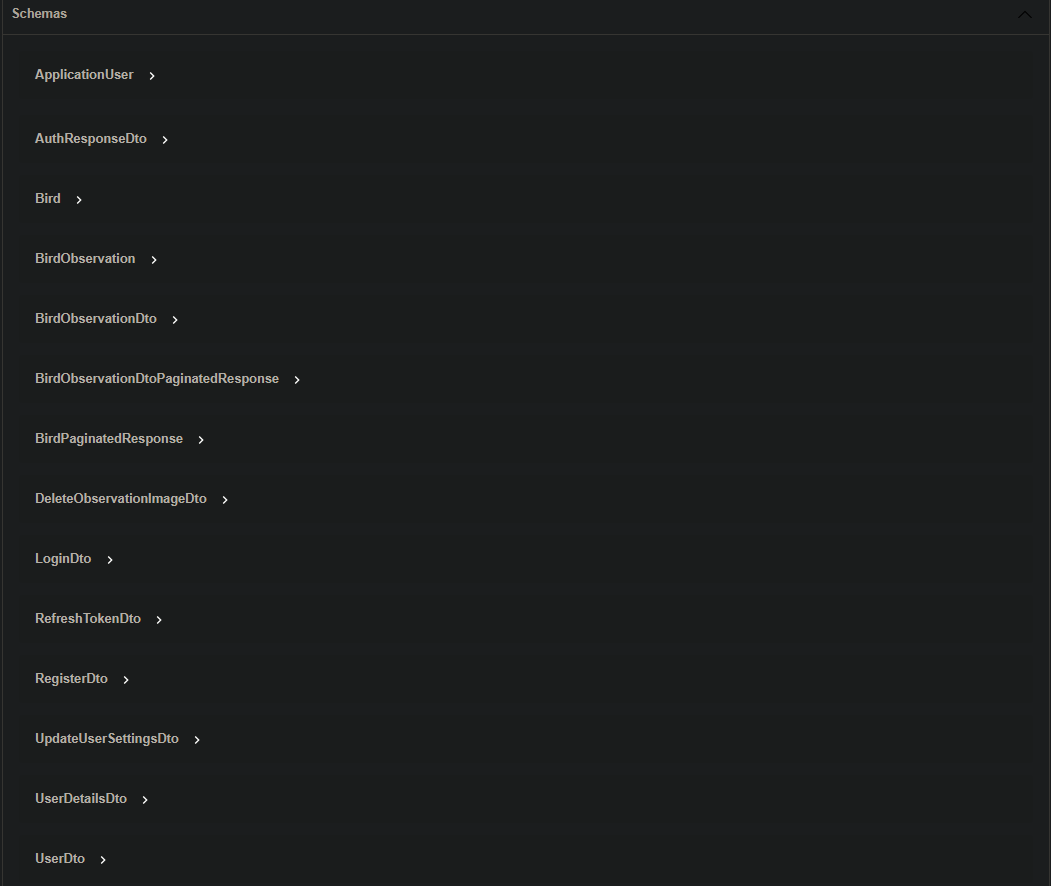
\includegraphics[width=1.0\textwidth]{/dodatekA/Swagger2.png}
	\caption{Interfejs Swagger struktury}
	\label{fig:swagger2}
\end{figure}

\begin{figure}[!htb]
	\centering
	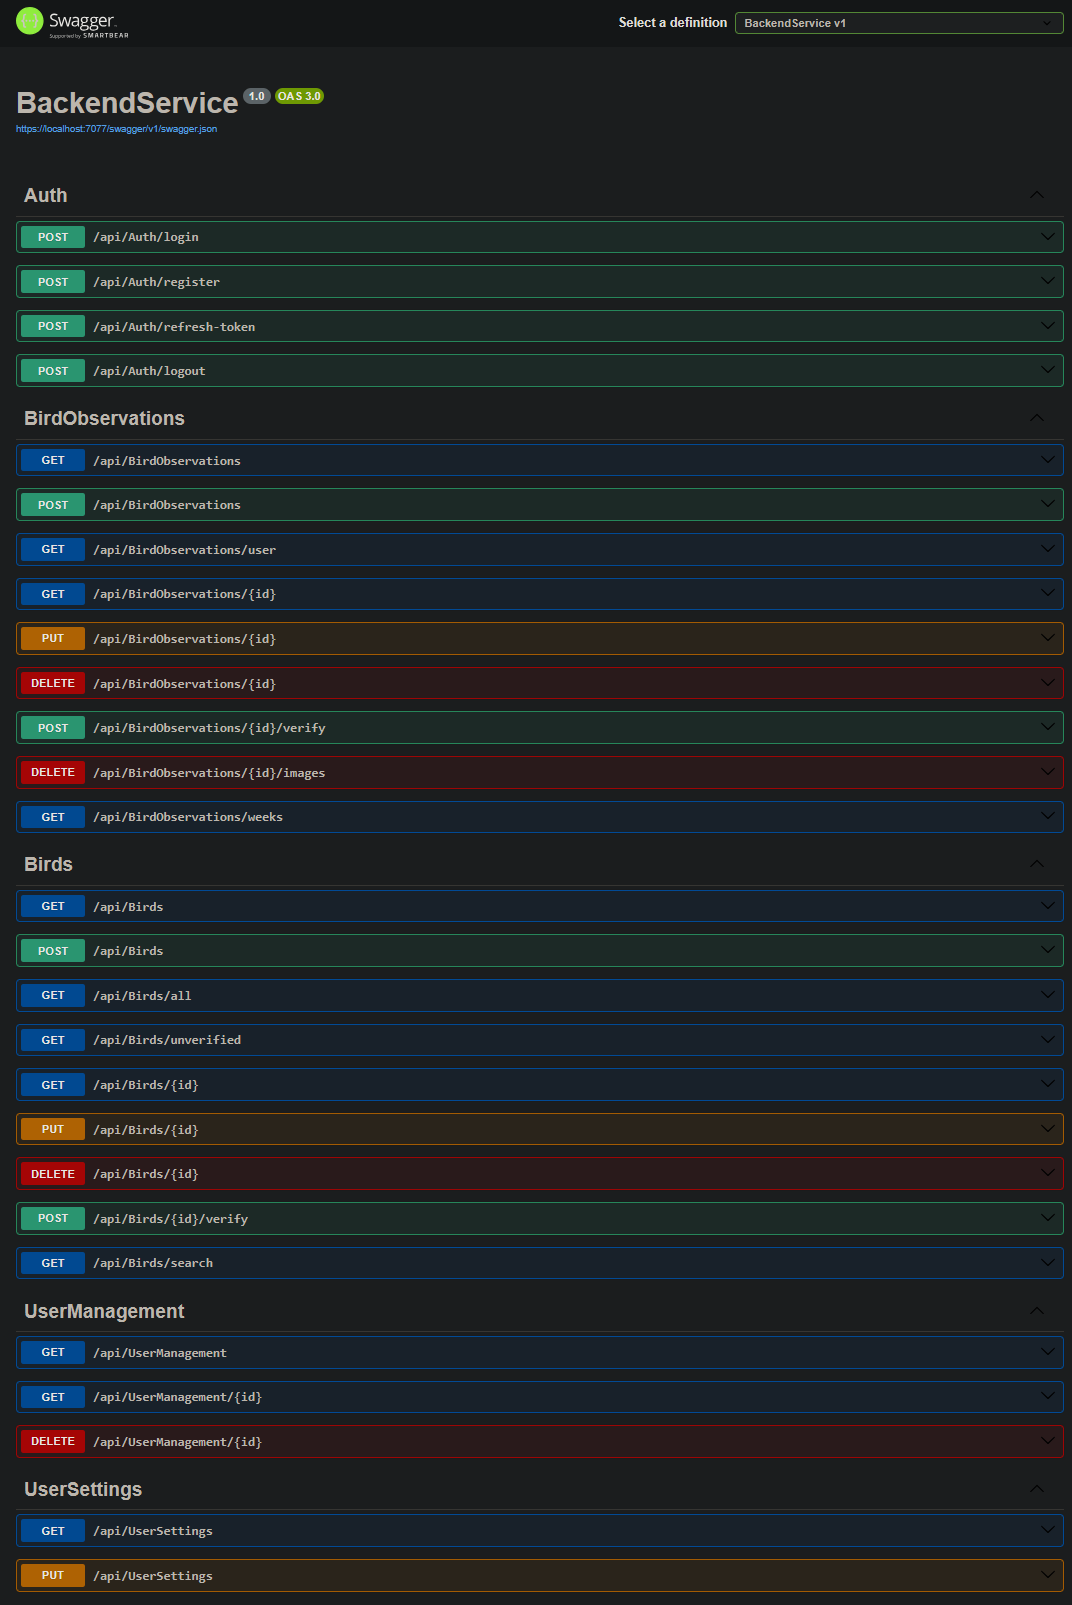
\includegraphics[width=1.0\textwidth]{/dodatekA/Swagger1.png}
	\caption{Interfejs Swagger endpointy}
	\label{fig:swagger1}
\end{figure} % conclusions.tex zawiera treść zakończenia/podsumowania pracy dyplomowej
\end{appendix}
%----------------------------------------------------------------------------------------
% Koniec dokumentu
\end{document}
